\begin{figure}[h]
\centering
\begin{tabular}{clc}
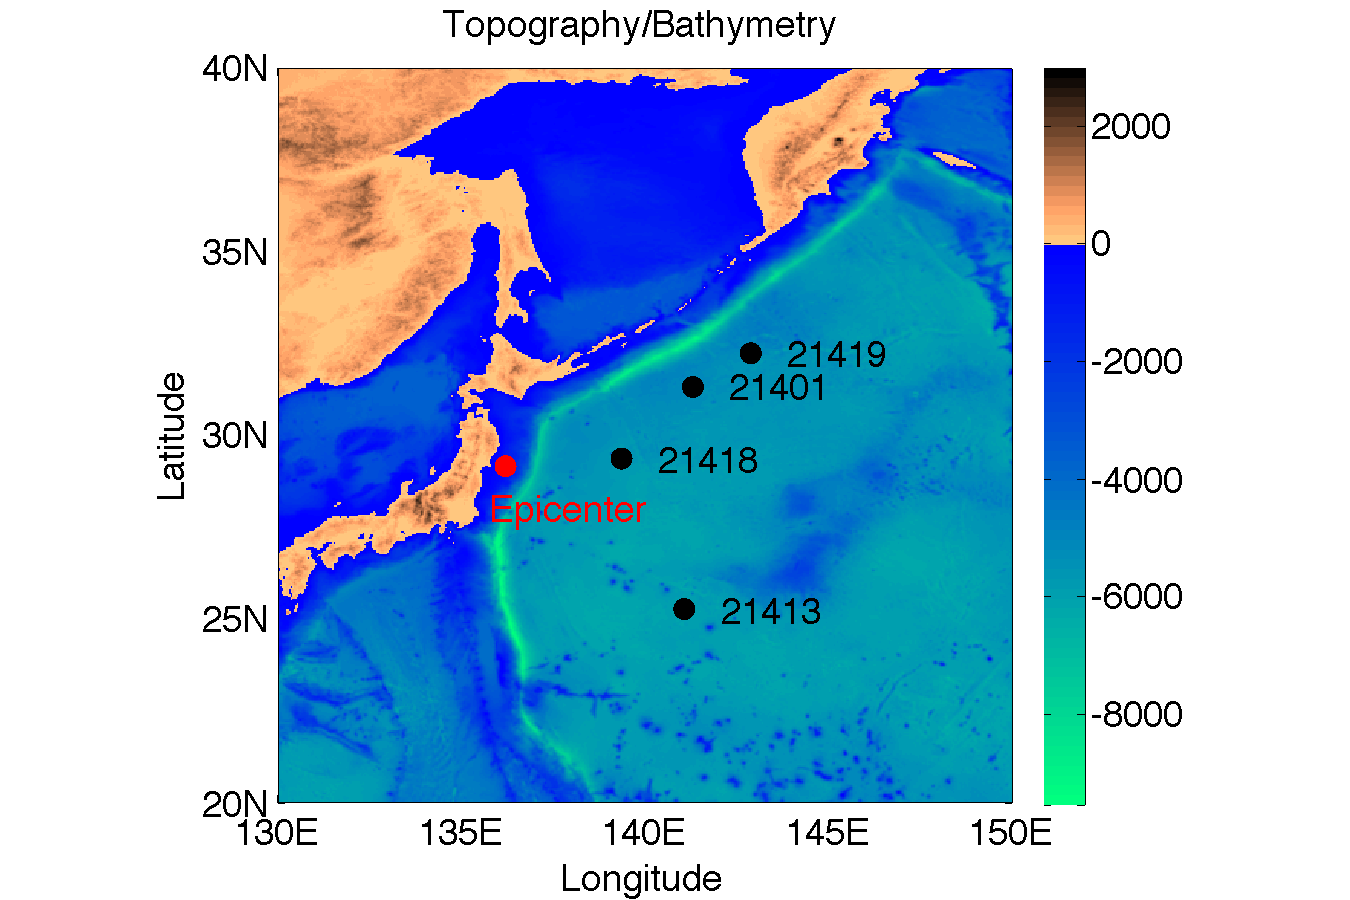
\includegraphics[width=0.45\textwidth]{./figures/topo.pdf}  &
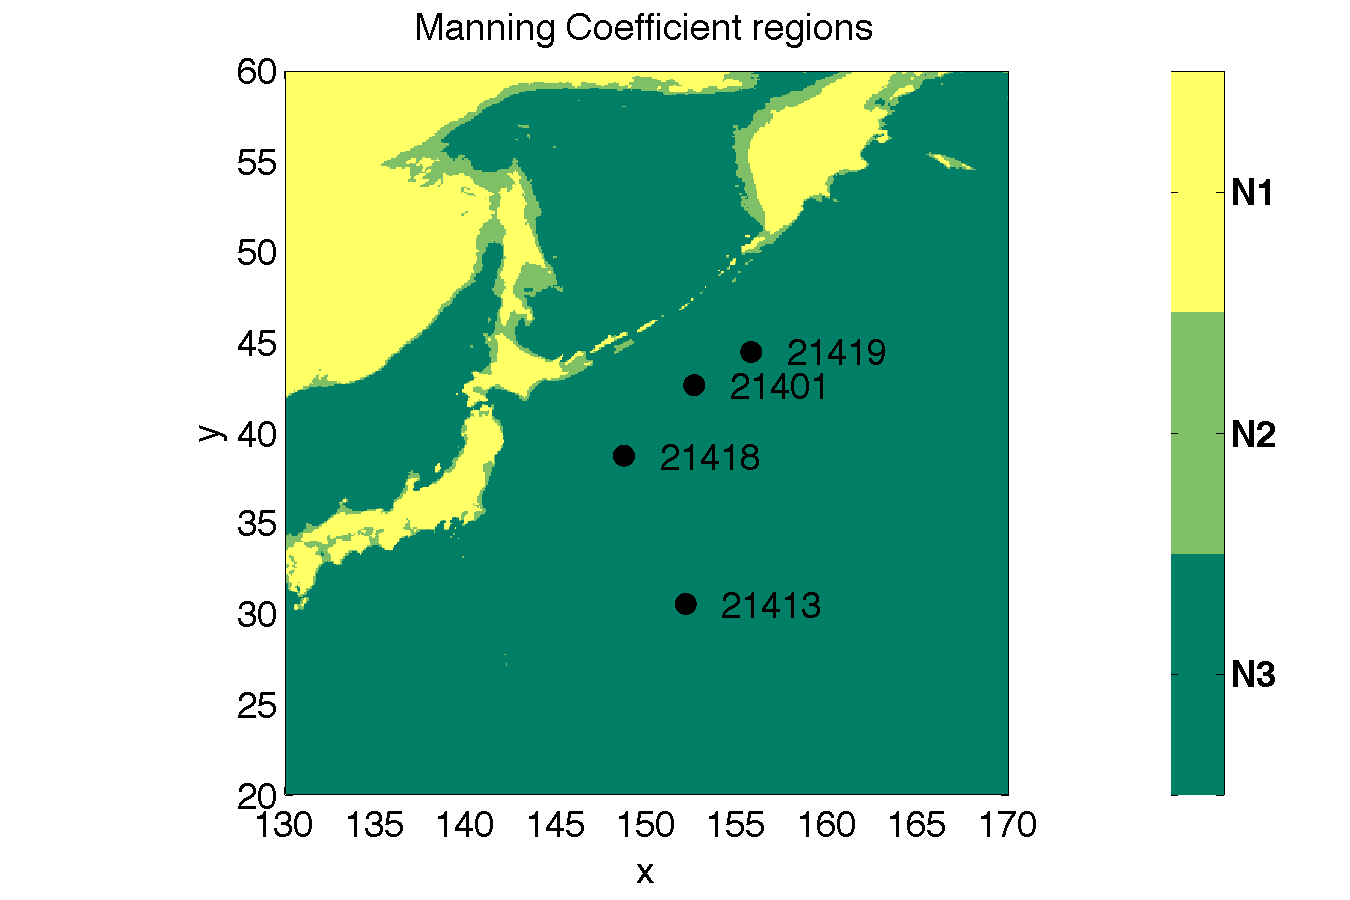
\includegraphics[width=0.45\textwidth]{./figures/coef.pdf} 
\label{setup}
\end{tabular}
\caption{Topography and gauge locations.}
\label{fig:setup}
\end{figure}
%%%%%%%%%%%%%%%%%%%%%%%%%%%%%%%%%%%%%%%%%%%%%%%%%%%%%%%%%%%%%%%%
\begin{figure}[h]      
\centering
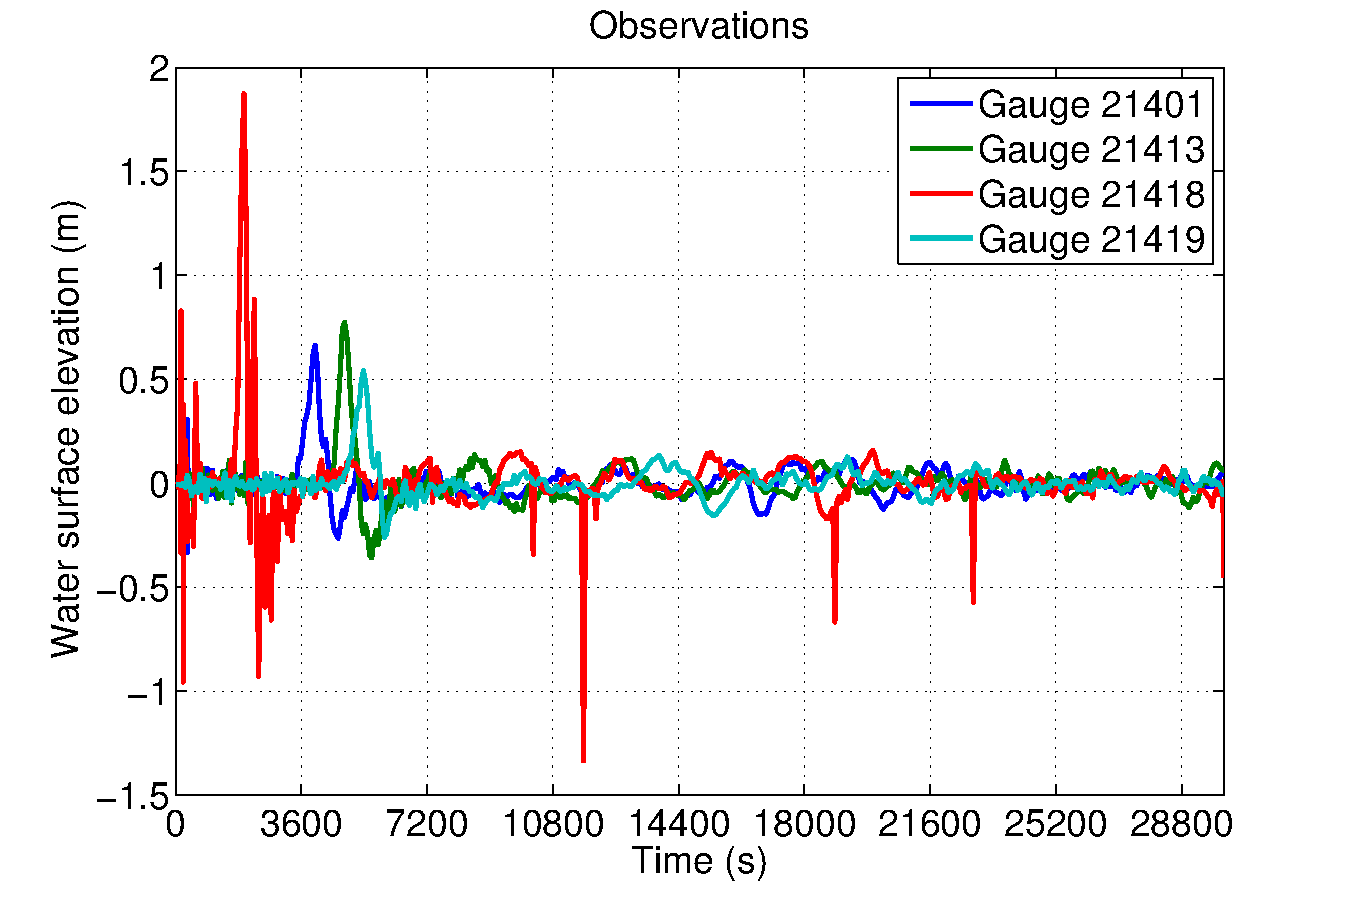
\includegraphics[width=0.6\textwidth]{./figures/obs.pdf}
\caption{Observed data of water surface elevation with time at four different gauges.}
\label{fig:obs}
\end{figure}  
%%%%%%%%%%%%%%%%%%%%%%%%%%%%%%%%%%%%%%%%%%%%%%%%%%%%%%%%%%%%%%%%
\begin{figure}[h]
\centering
\begin{tabular}{clc}        
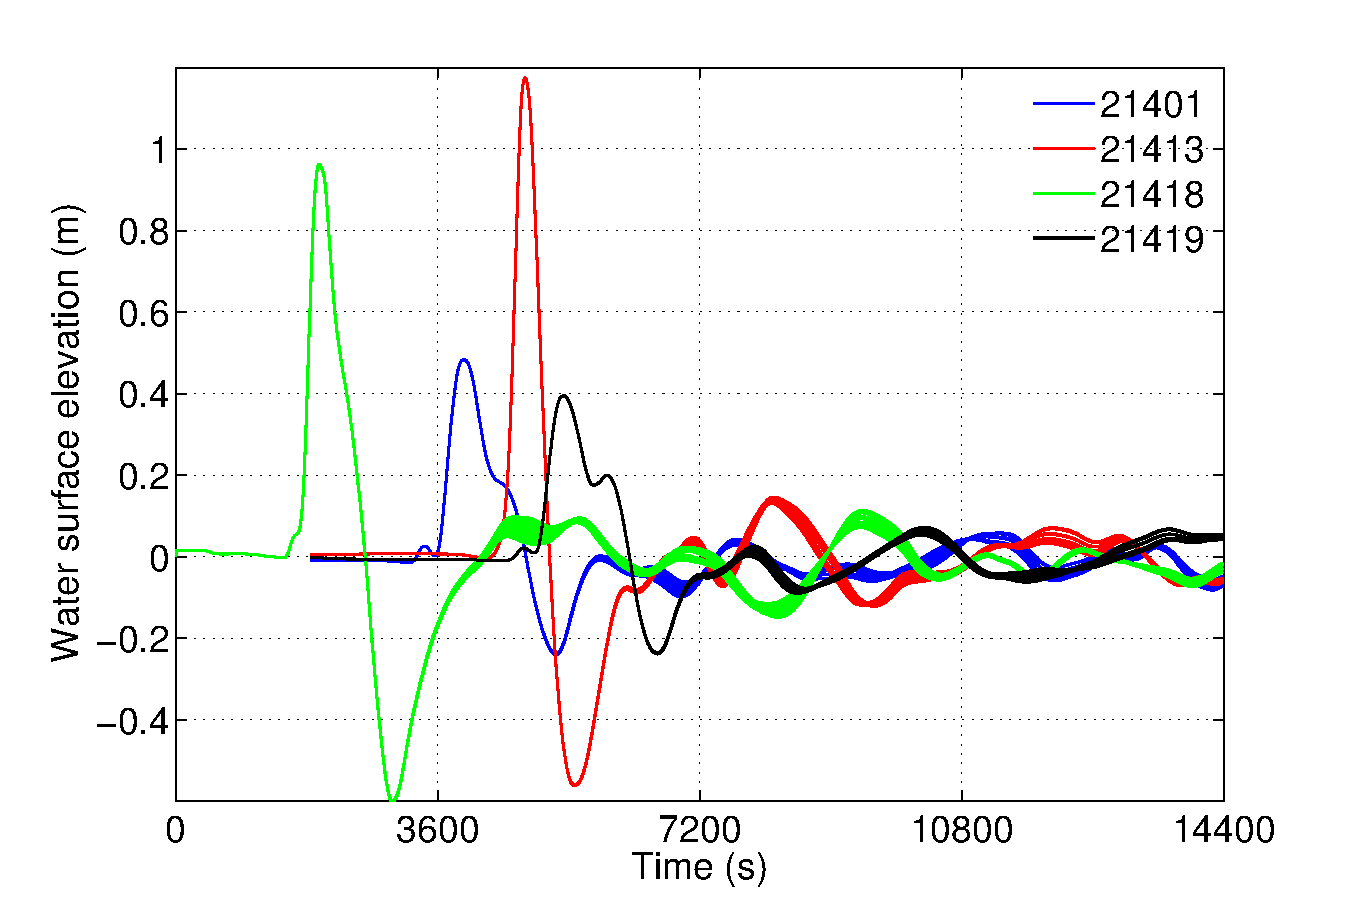
\includegraphics[width=0.6\textwidth]{./figures/rlzs_gauges.pdf} 
\end{tabular}
\caption{125 Geoclaw realizations at different gauge locations.}
\label{fig:rlzs}
\end{figure}
%%%%%%%%%%%%%%%%%%%%%%%%%%%%%%%%%%%%%%%%%%%%%%%%%%%%%%%%%%%%%%%%

\begin{figure}[h]
\centering
\begin{tabular}{clc}        
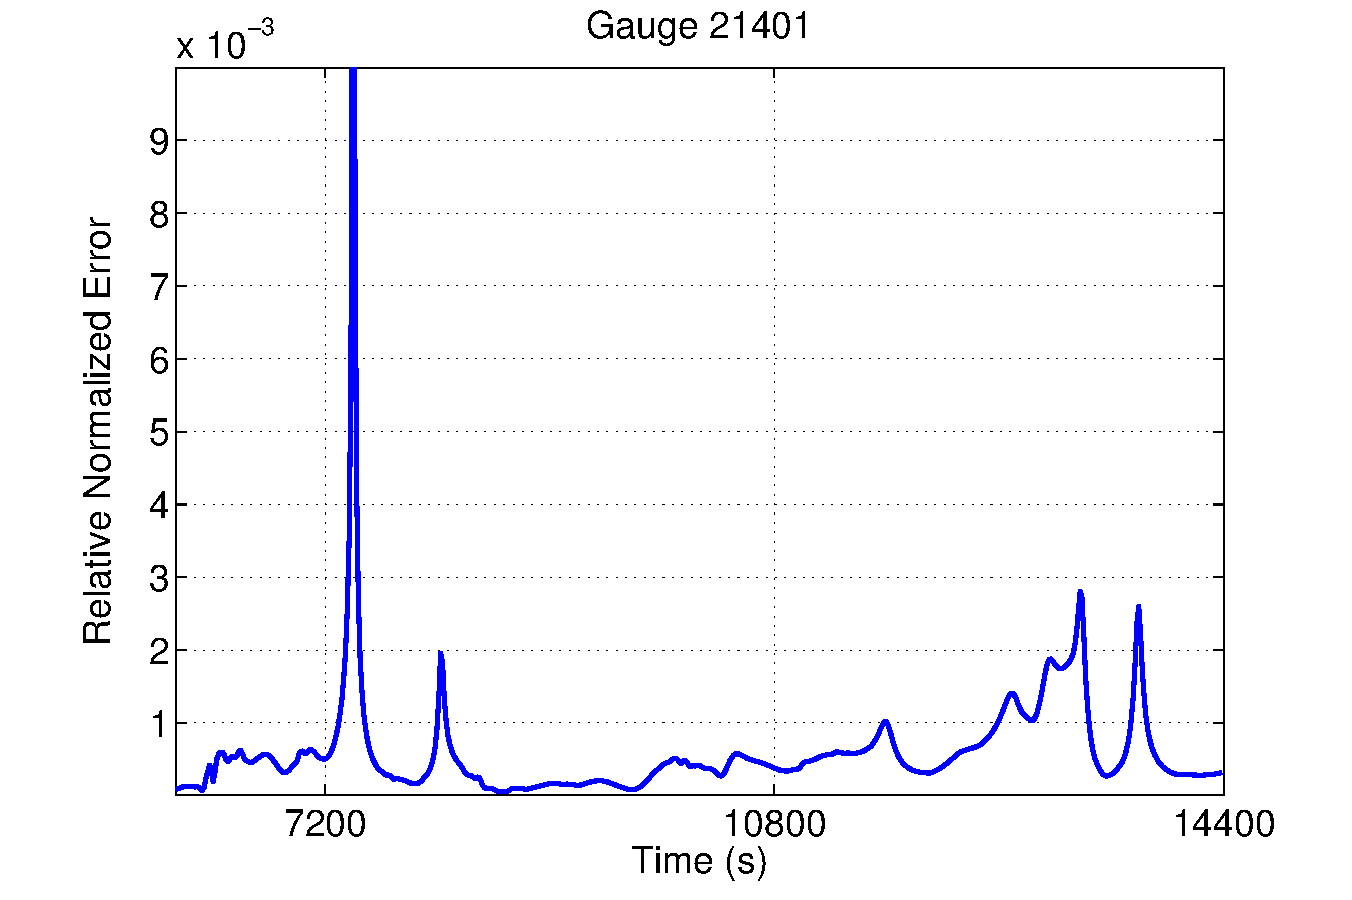
\includegraphics[width=0.5\textwidth]{./figures/error_gauge1.pdf} &
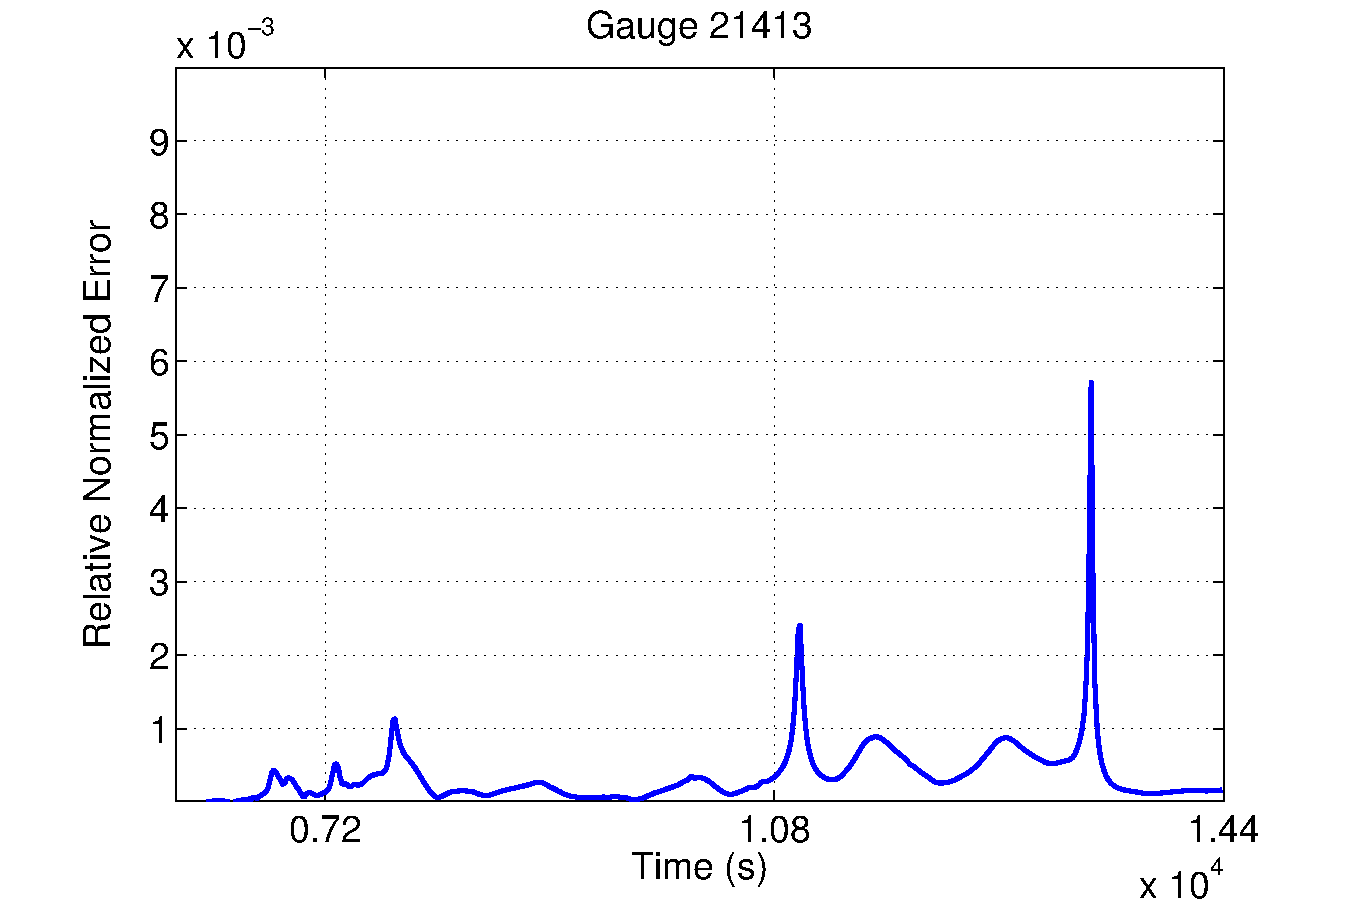
\includegraphics[width=0.5\textwidth]{./figures/error_gauge2.pdf} \\
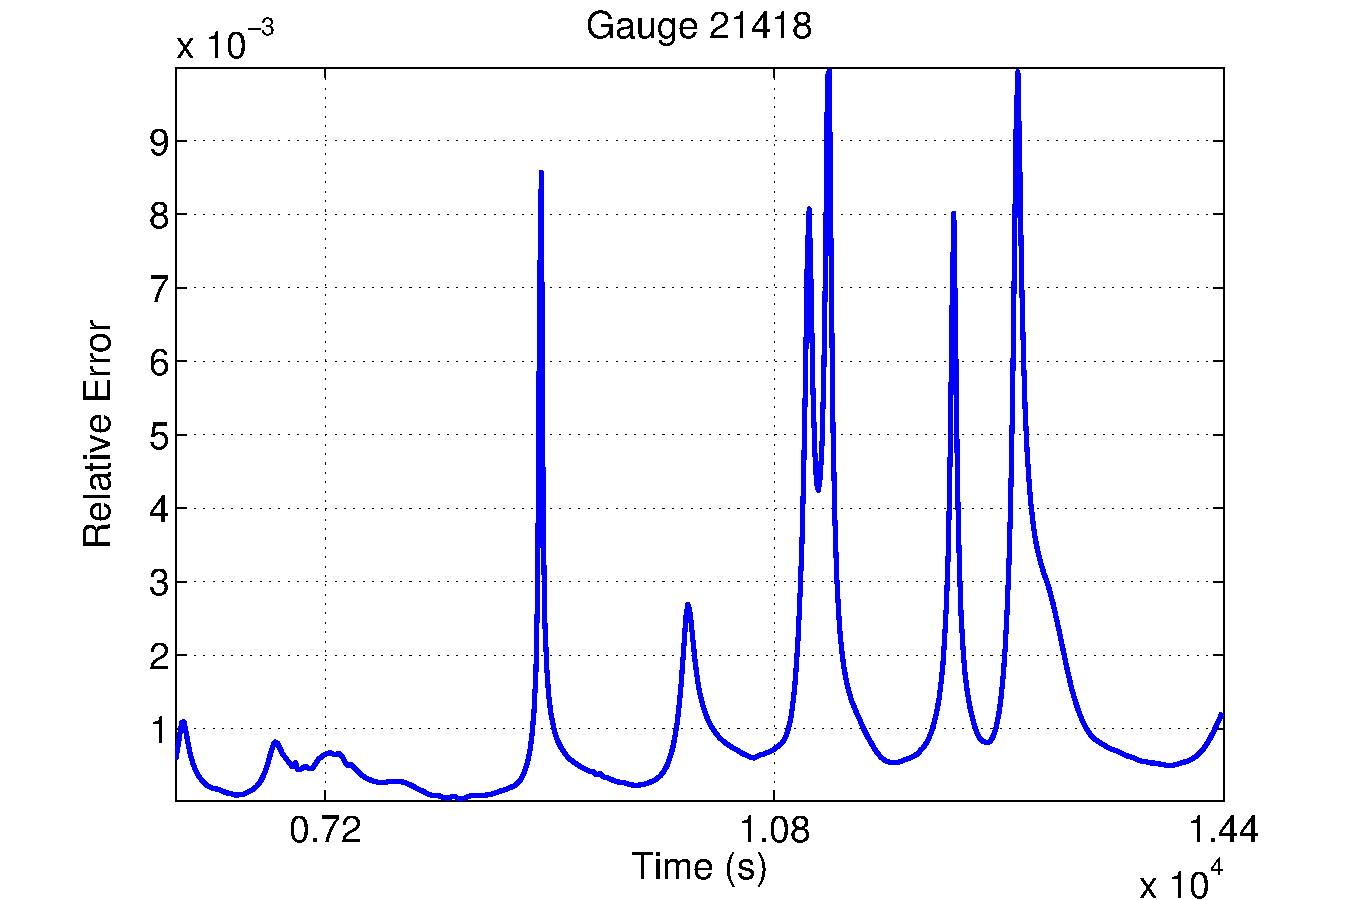
\includegraphics[width=0.5\textwidth]{./figures/error_gauge3.pdf} &
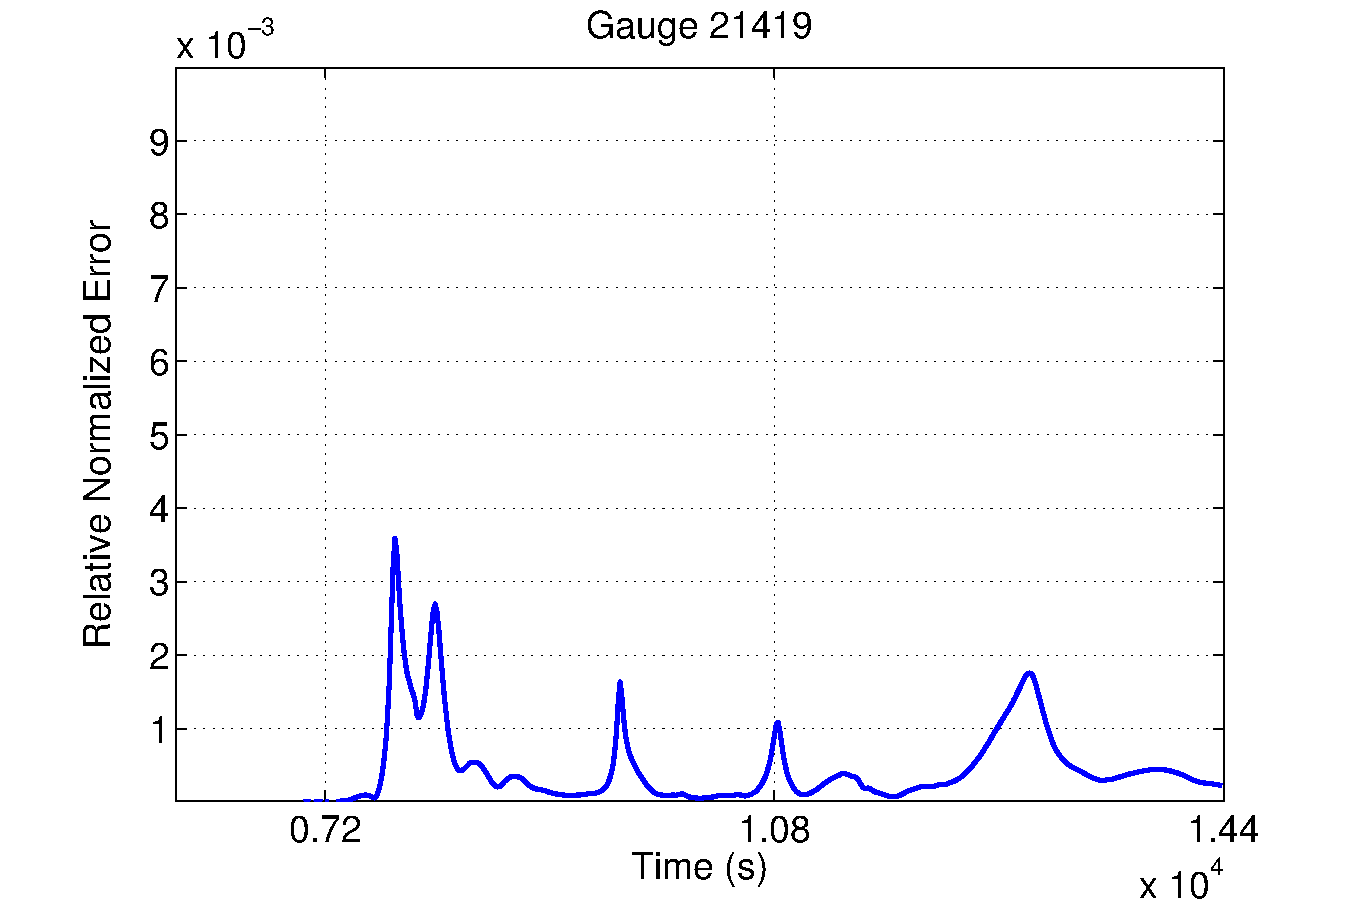
\includegraphics[width=0.5\textwidth]{./figures/error_gauge4.pdf} 

\end{tabular}
\caption{125 Geoclaw realizations at different gauge locations.}
\label{fig:error}
\end{figure}   
%%%%%%%%%%%%%%%%%%%%%%%%%%%%%%%%%%%%%%%%%%%%%%%%%%%%%%%%%%%%%%%%
\begin{figure}[h]
\centering

\begin{tabular}{clcl}
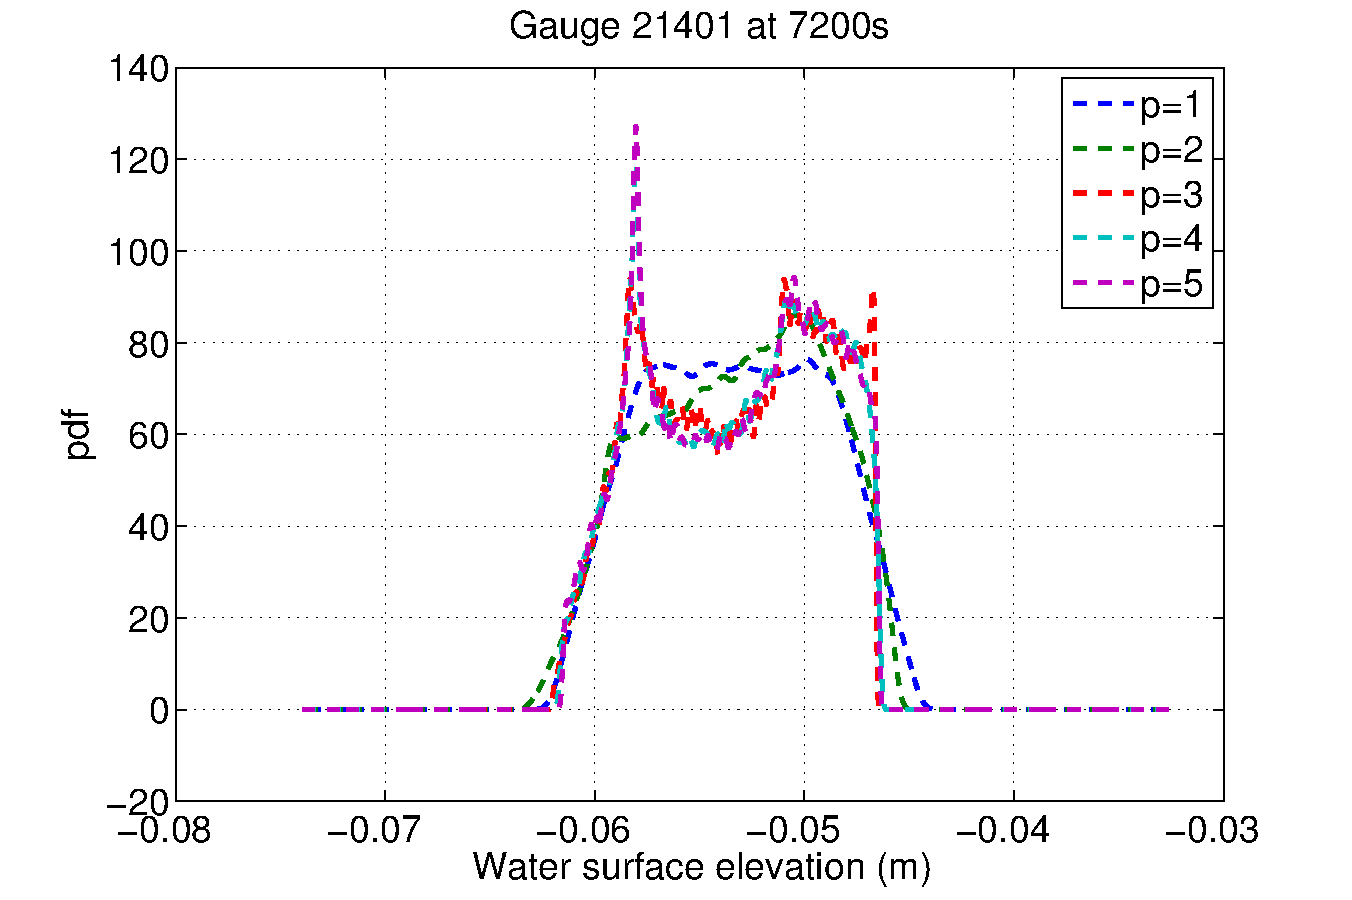
\includegraphics[width=0.5\textwidth]{./figures/pdfs1_2.pdf} &
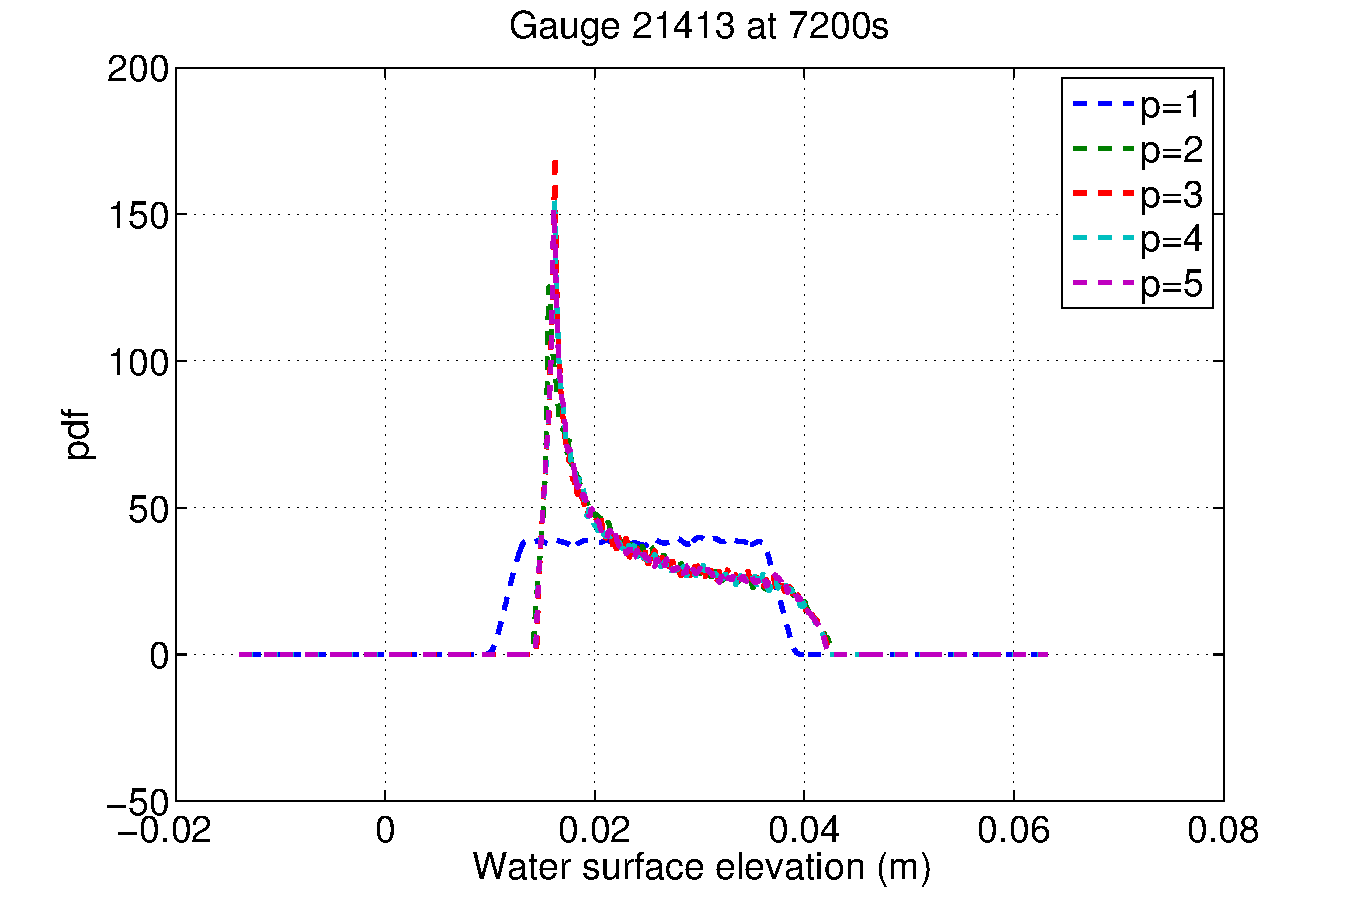
\includegraphics[width=0.5\textwidth]{./figures/pdfs2_2.pdf} \\
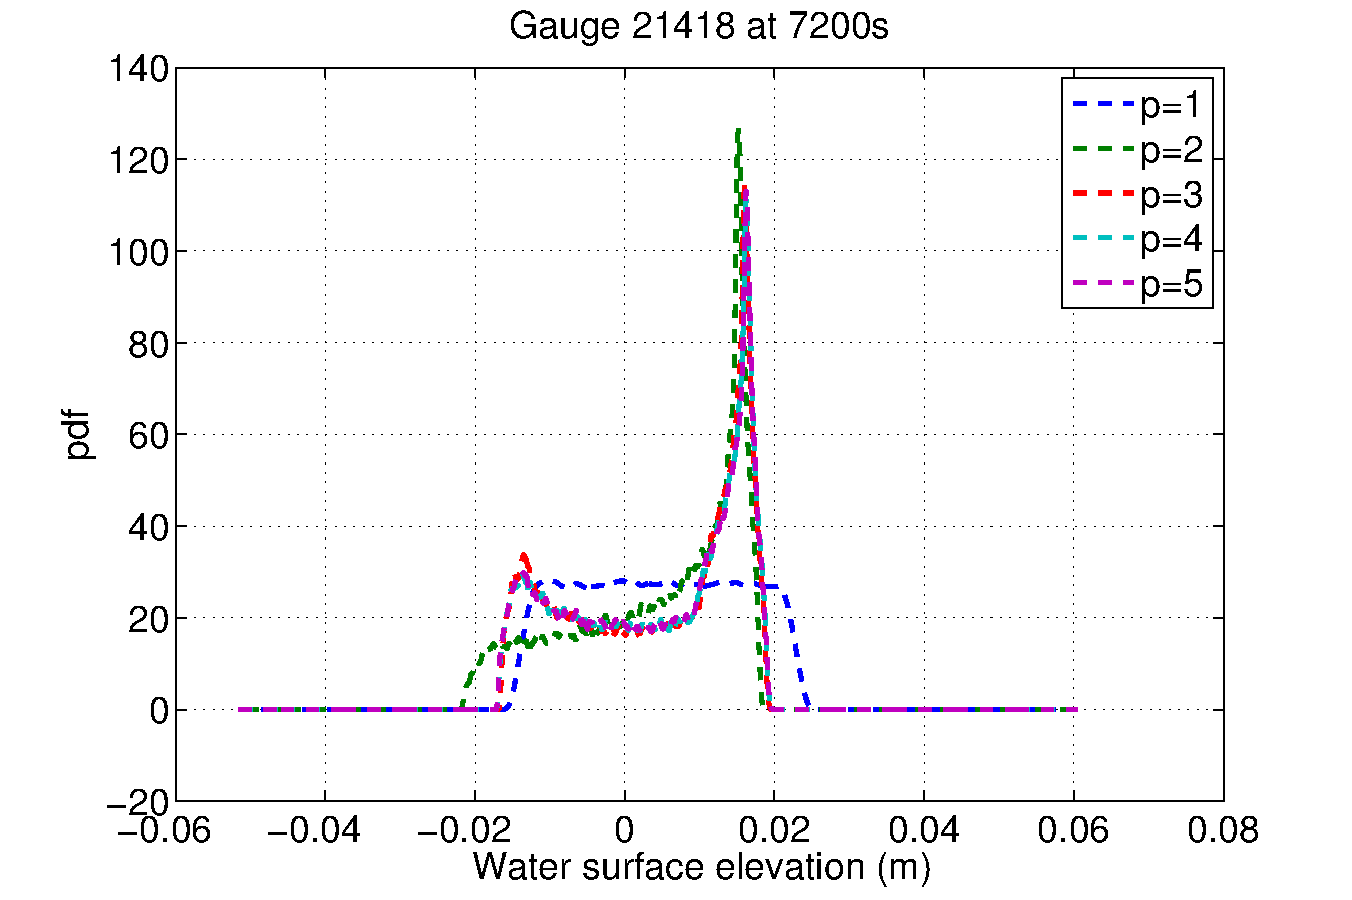
\includegraphics[width=0.5\textwidth]{./figures/pdfs3_2.pdf} &
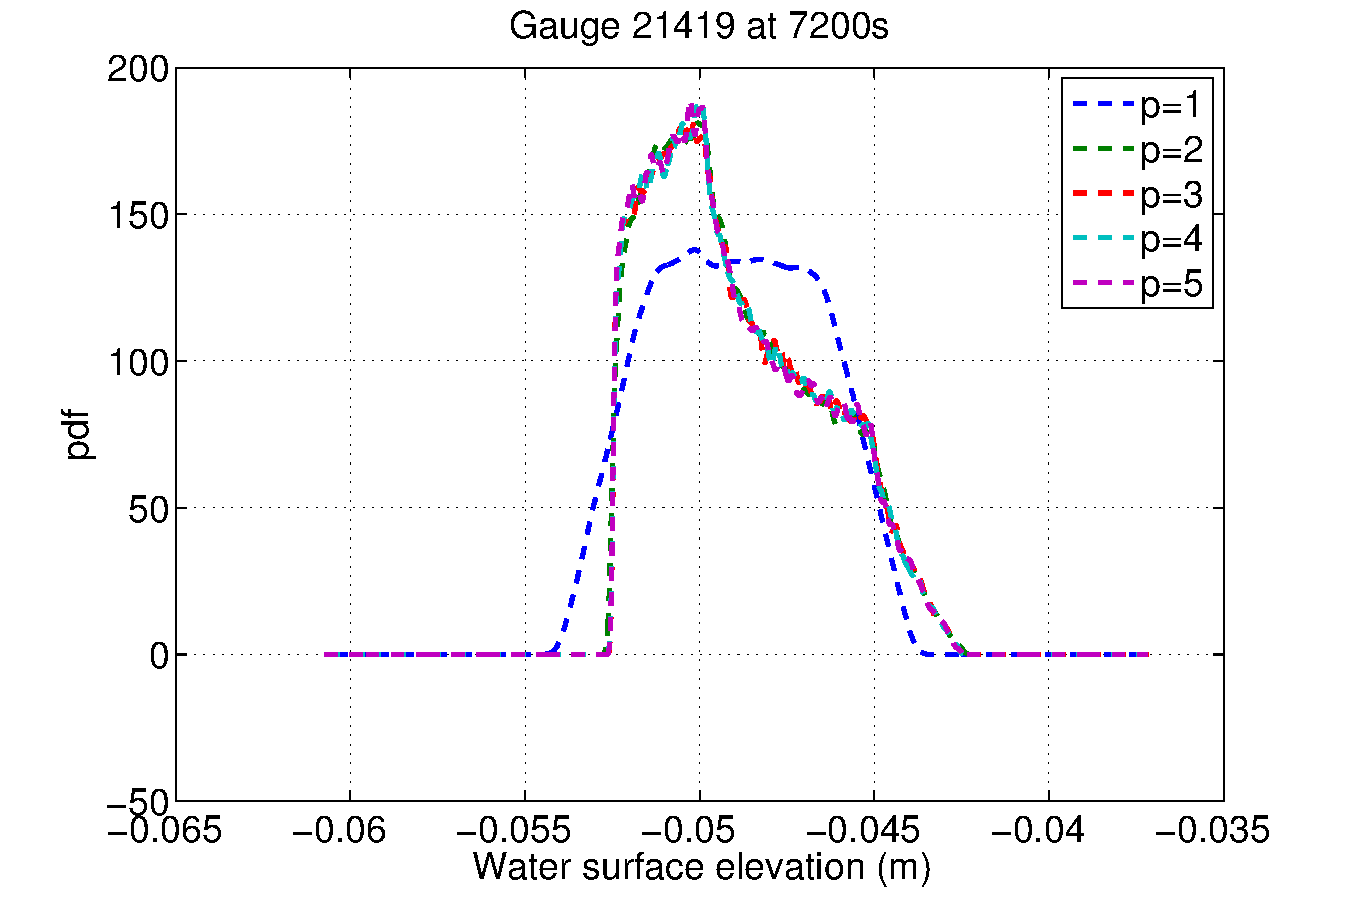
\includegraphics[width=0.5\textwidth]{./figures/pdfs4_2.pdf}
\end{tabular}
\caption{pdf of water surface elevation at the different gauge locations at t = 7200 s.}
\label{fig:pdfs2}
\end{figure}
%%%%%%%%%%%%%%%%%%%%%%%%%%%%%%%%%%%%%%%%%%%%%%%%%%%%%%%%%%%%%%%%
\begin{figure}[h]
\centering
\begin{tabular}{clc}
        
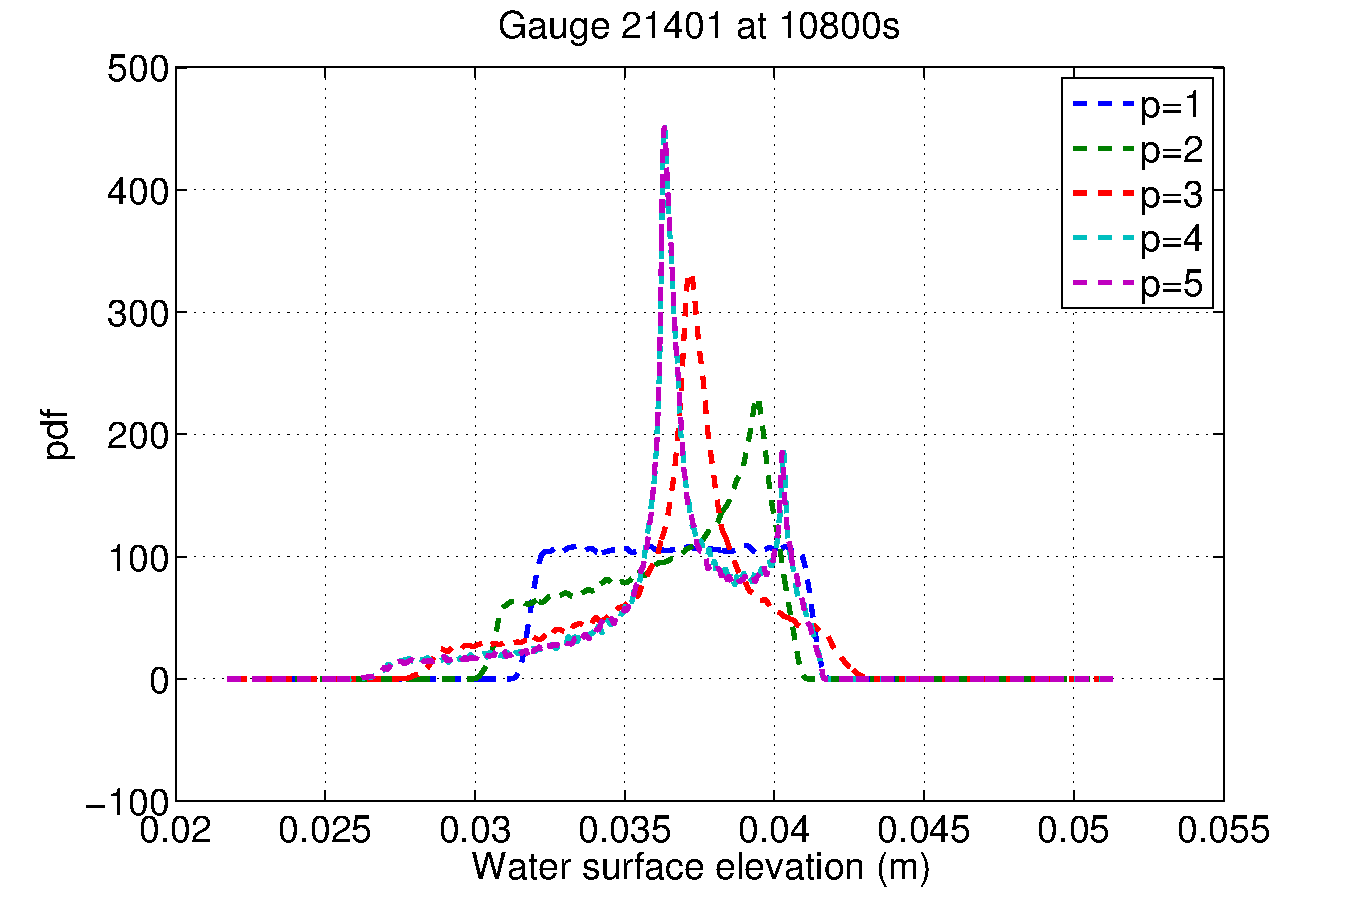
\includegraphics[width=0.5\textwidth]{./figures/pdfs1_3.pdf} &
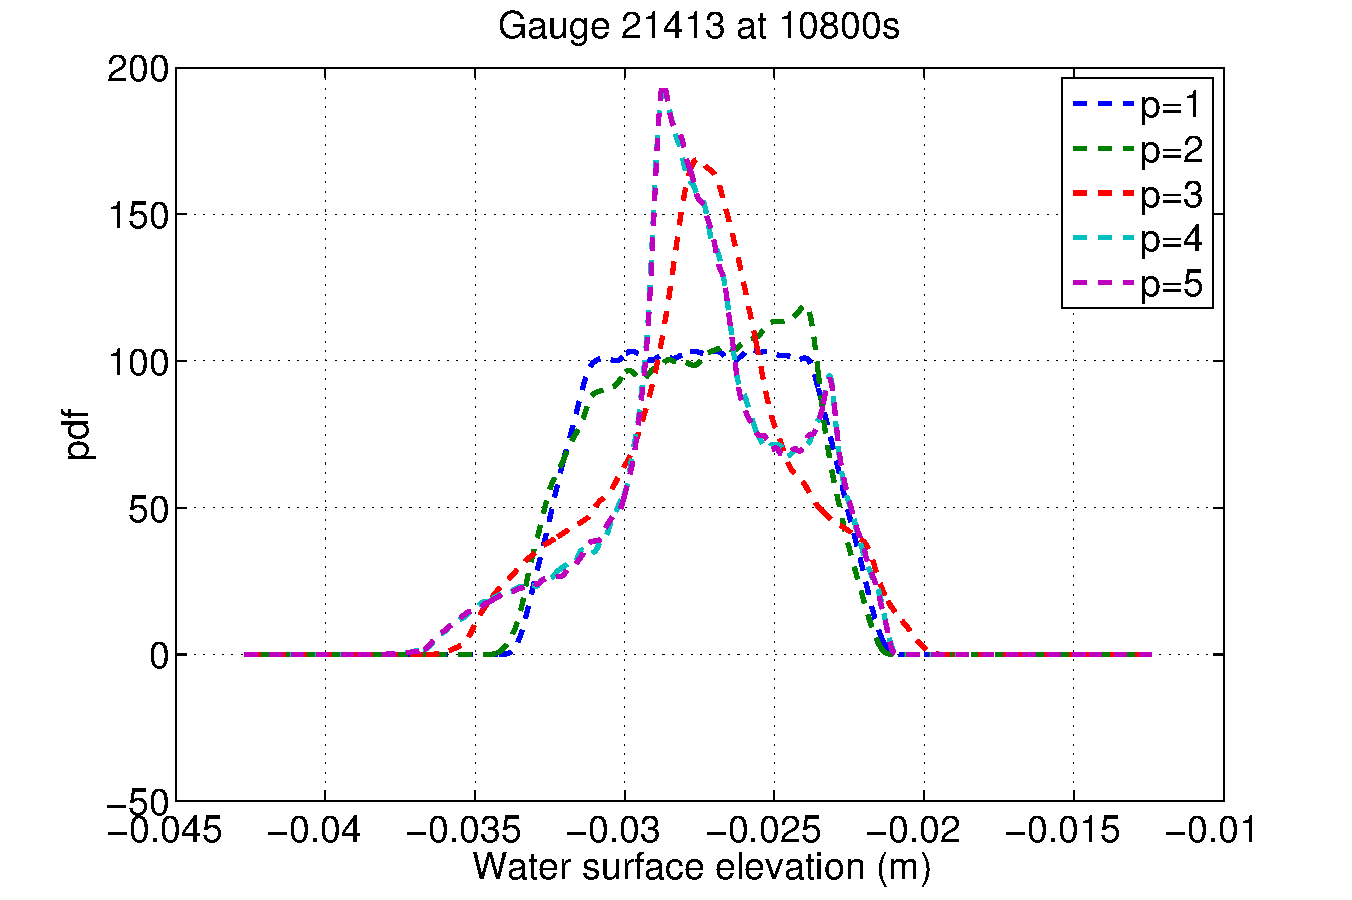
\includegraphics[width=0.5\textwidth]{./figures/pdfs2_3.pdf} \\
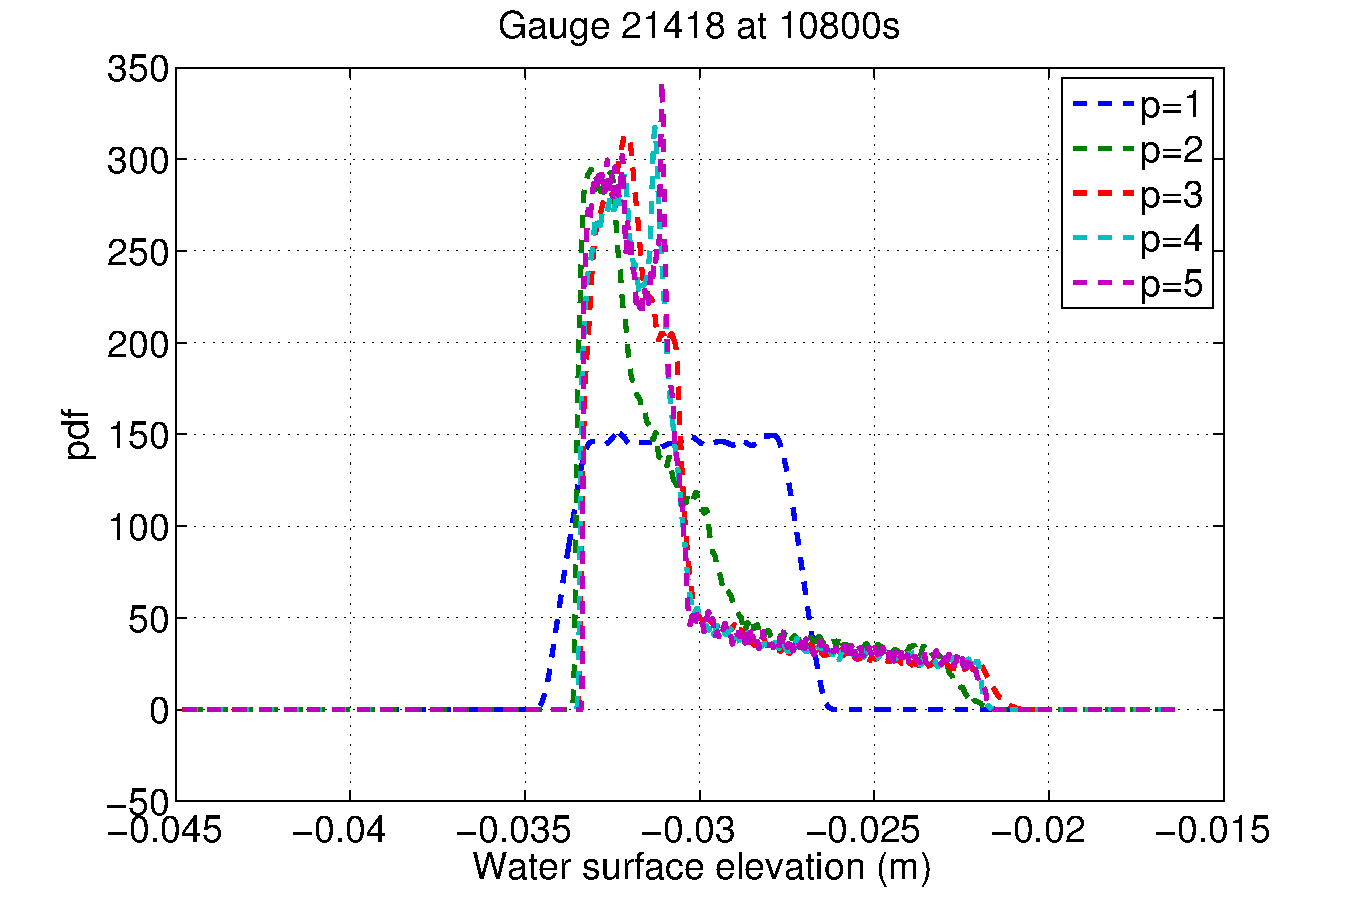
\includegraphics[width=0.5\textwidth]{./figures/pdfs3_3.pdf} &
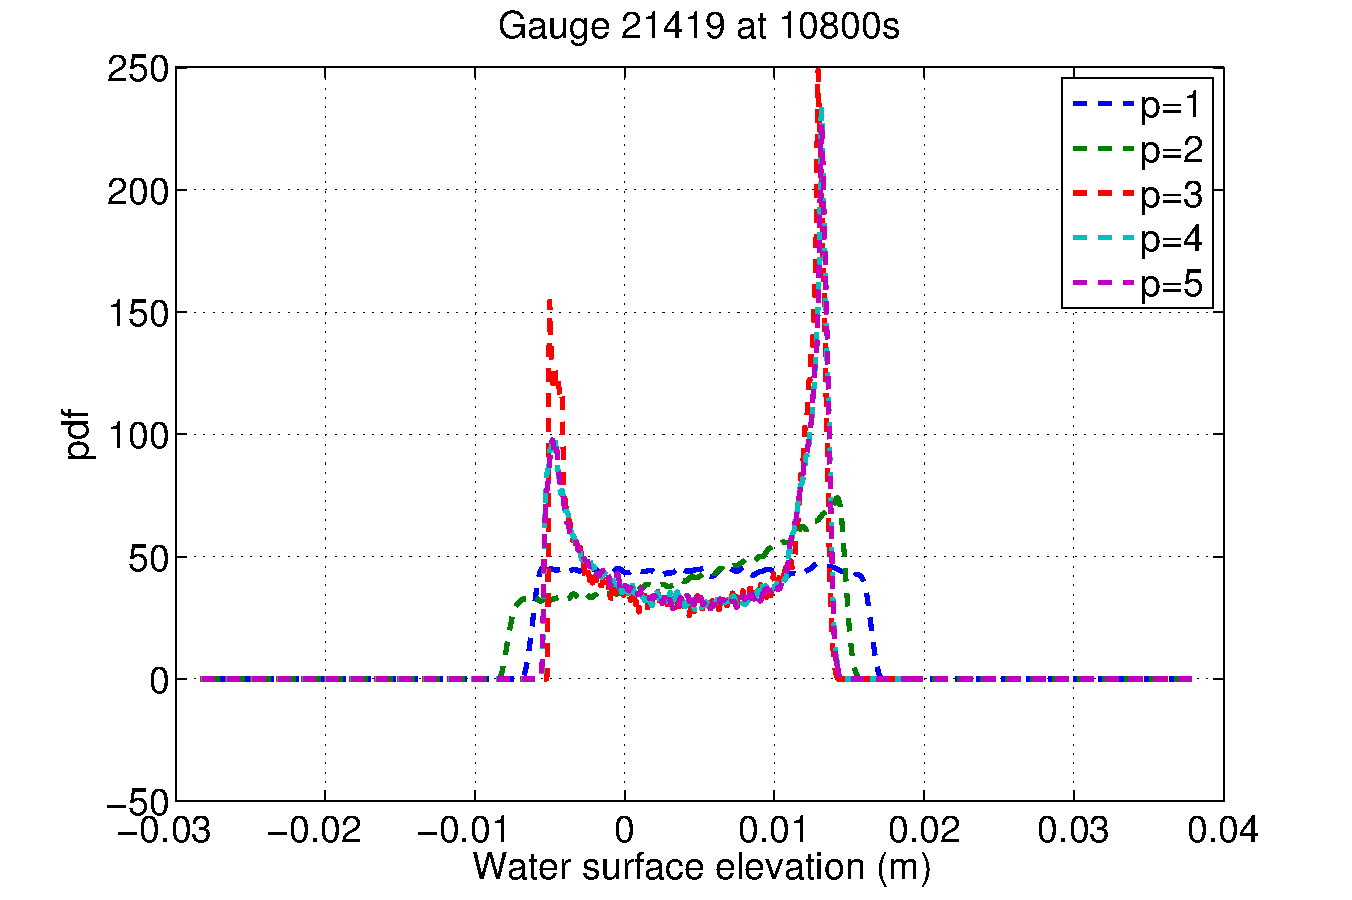
\includegraphics[width=0.5\textwidth]{./figures/pdfs4_3.pdf}
\end{tabular}
\caption{pdf of water surface elevation at the different gauge locations at t = 10800 s.}
\label{fig:pdfs3}
\end{figure}
%%%%%%%%%%%%%%%%%%%%%%%%%%%%%%%%%%%%%%%%%%%%%%%%%%%%%%%%%%%%%%%%
\begin{figure}[h]
\begin{tabular}{clc}
        
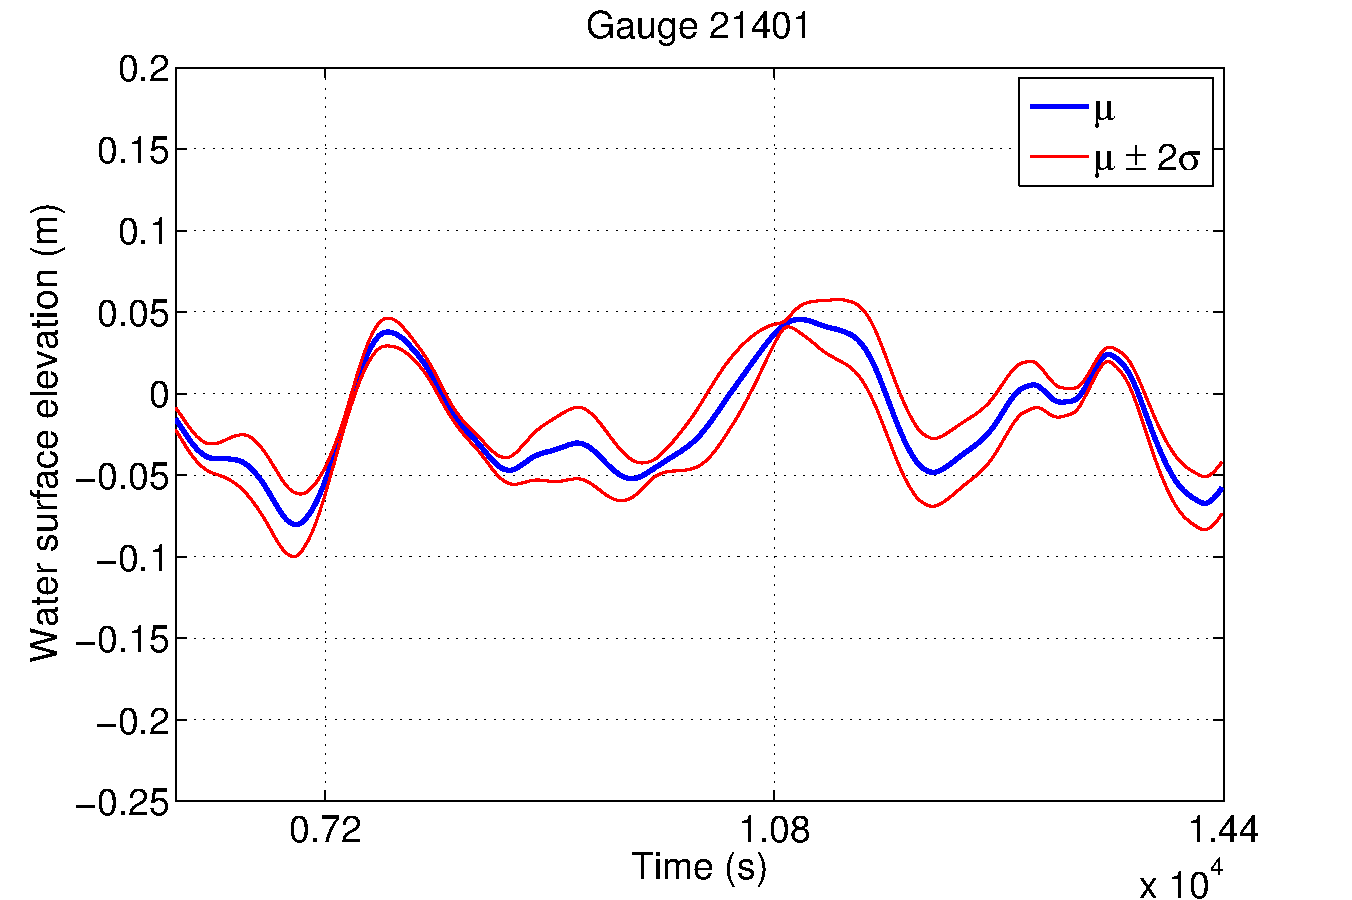
\includegraphics[width=0.475\textwidth]{./figures/musigma1.pdf} &
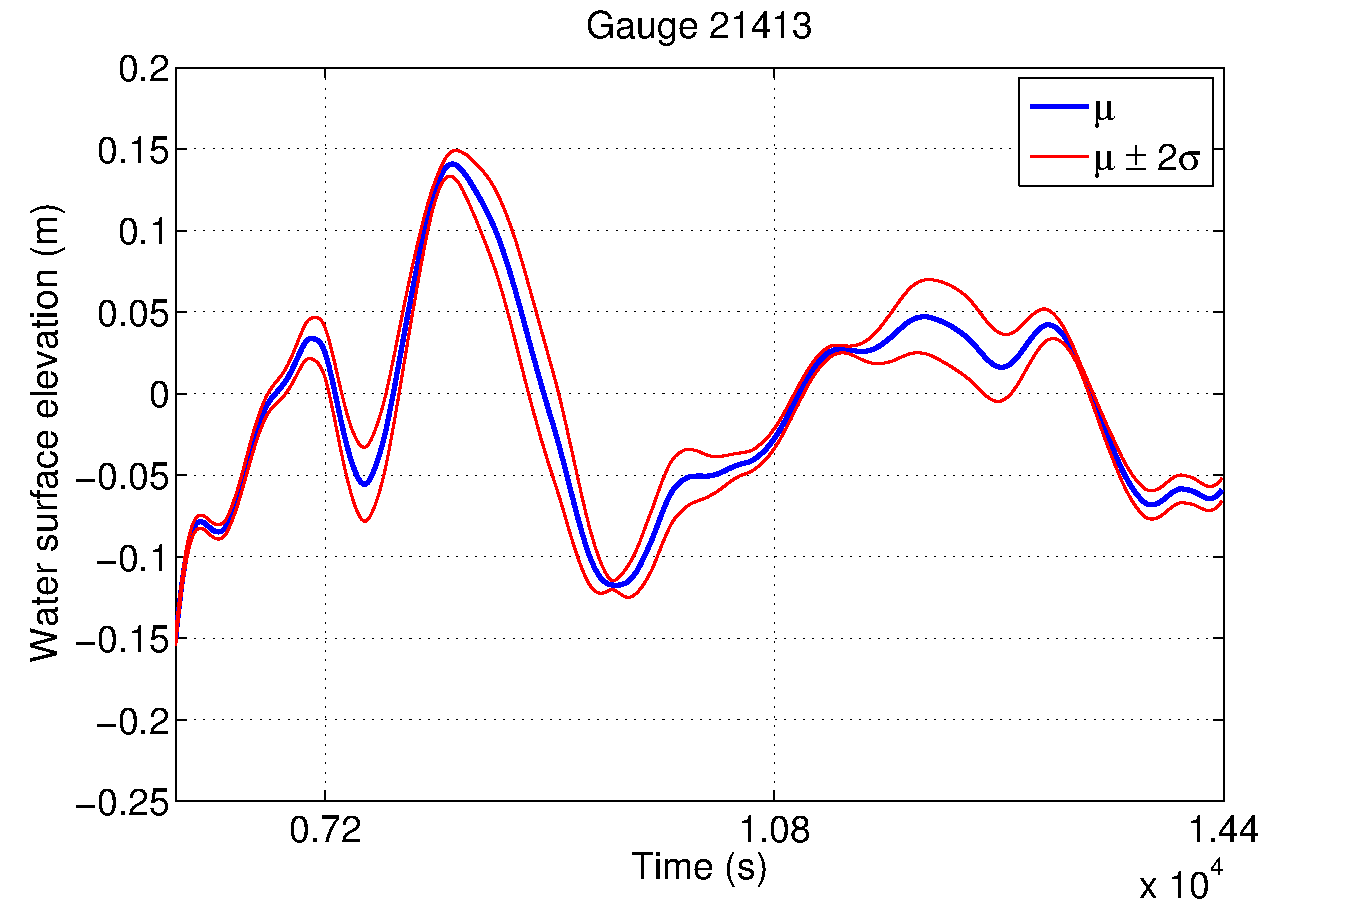
\includegraphics[width=0.475\textwidth]{./figures/musigma2.pdf} \\
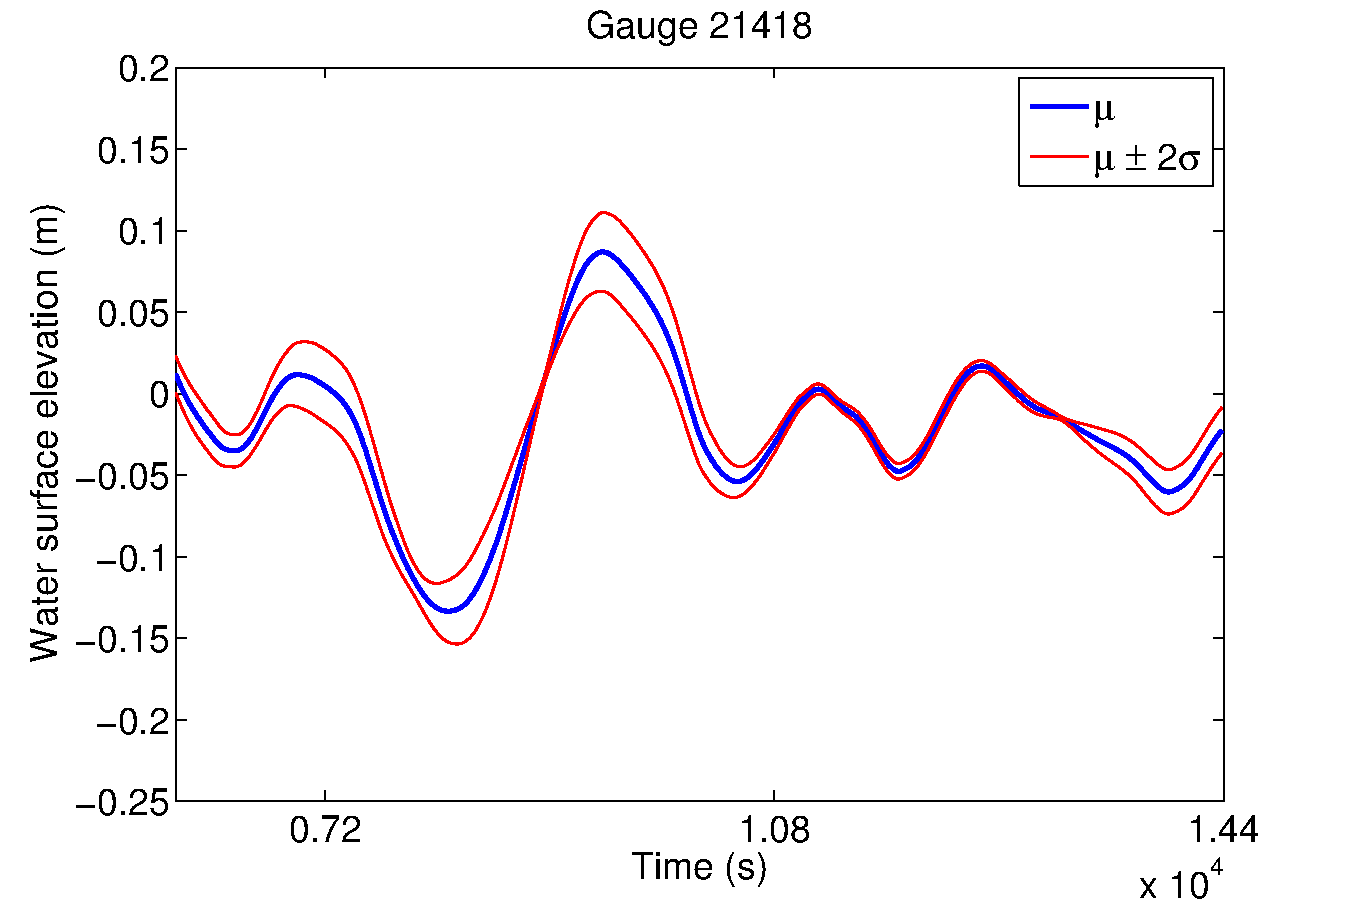
\includegraphics[width=0.475\textwidth]{./figures/musigma3.pdf} &
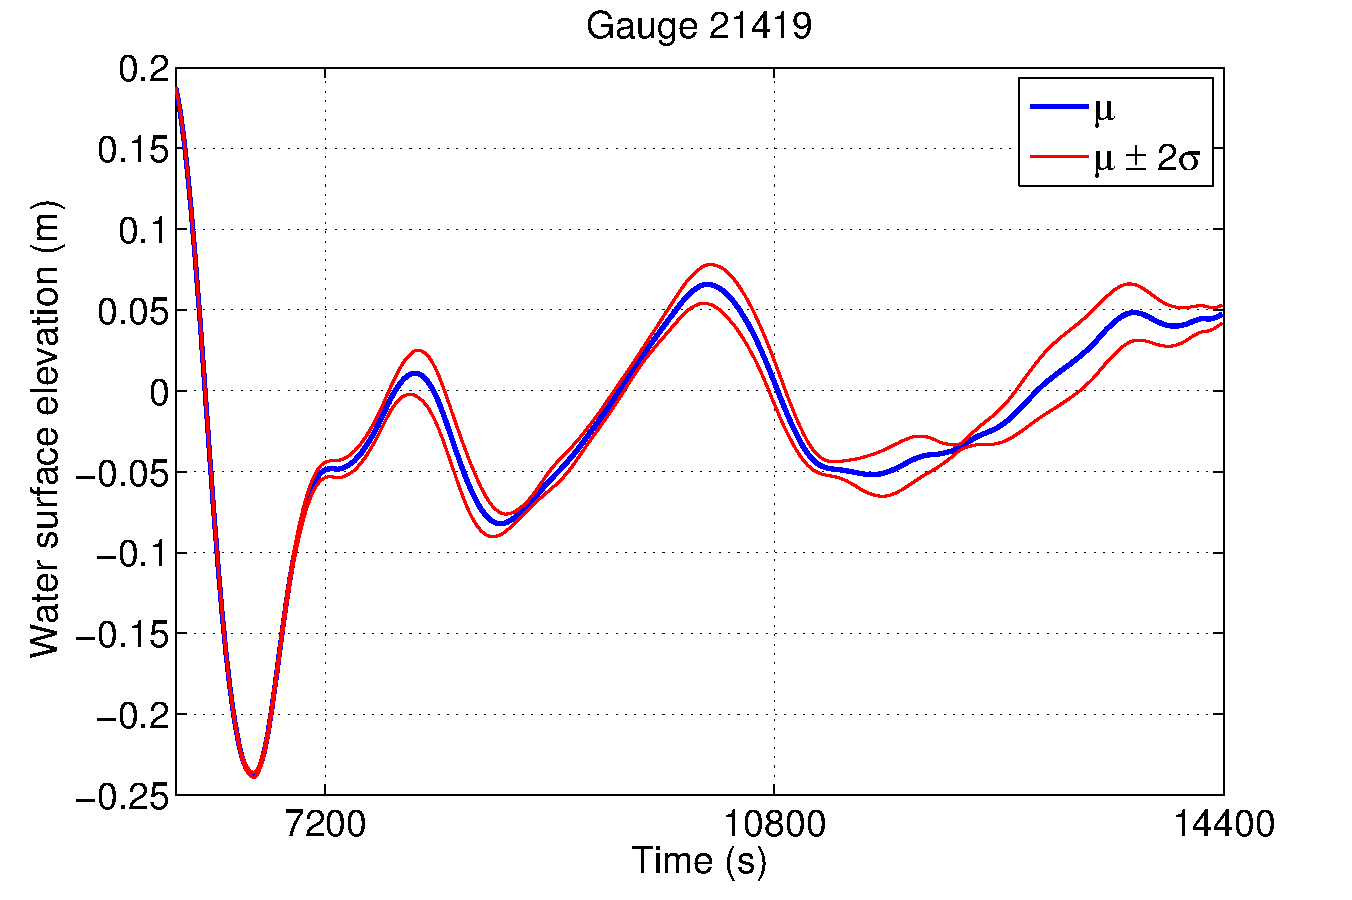
\includegraphics[width=0.475\textwidth]{./figures/musigma4.pdf}
\end{tabular}
\caption{Evolution of PC mean water surface elevation at different gauge locations.}
\label{fig:ave}
\end{figure}
%%%%%%%%%%%%%%%%%%%%%%%%%%%%%%%%%%%%%%%%%%%%%%%%%%%%%%%%%%%%%%%%

\begin{figure}[h]
\begin{tabular}{clc}
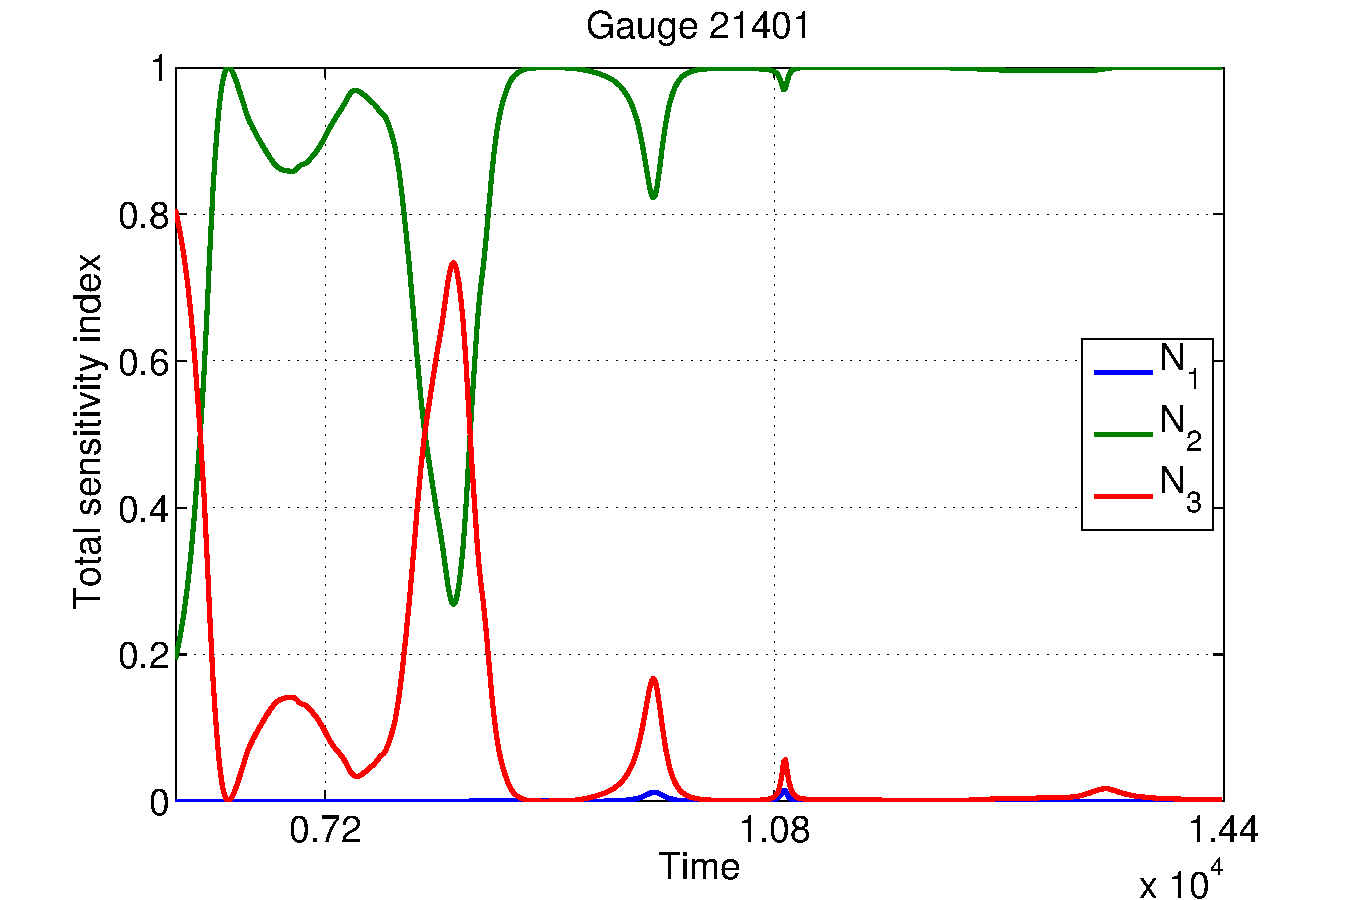
\includegraphics[width=0.475\textwidth]{./figures/sens1.pdf} &
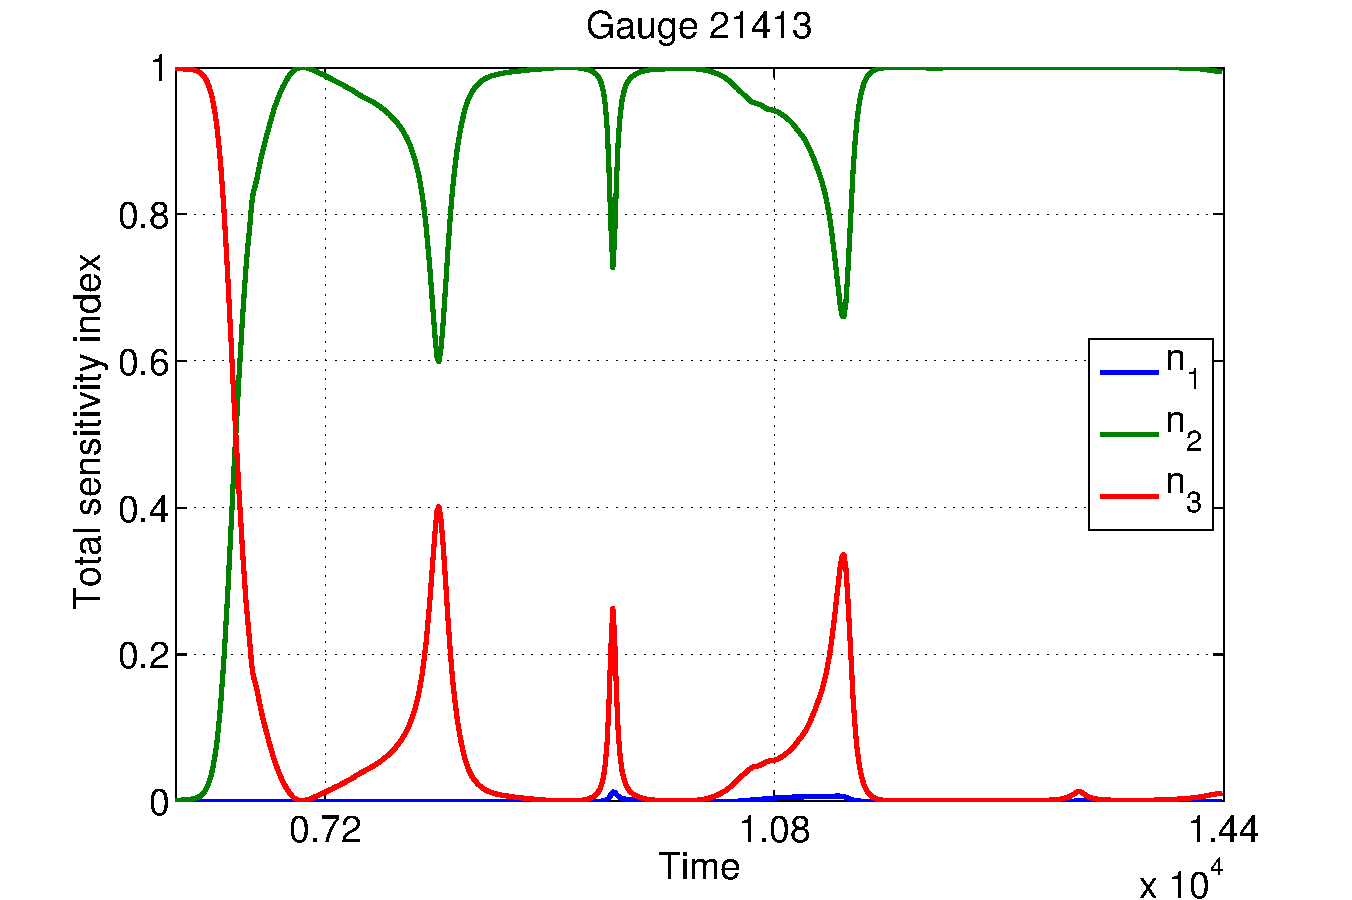
\includegraphics[width=0.475\textwidth]{./figures/sens2.pdf} \\
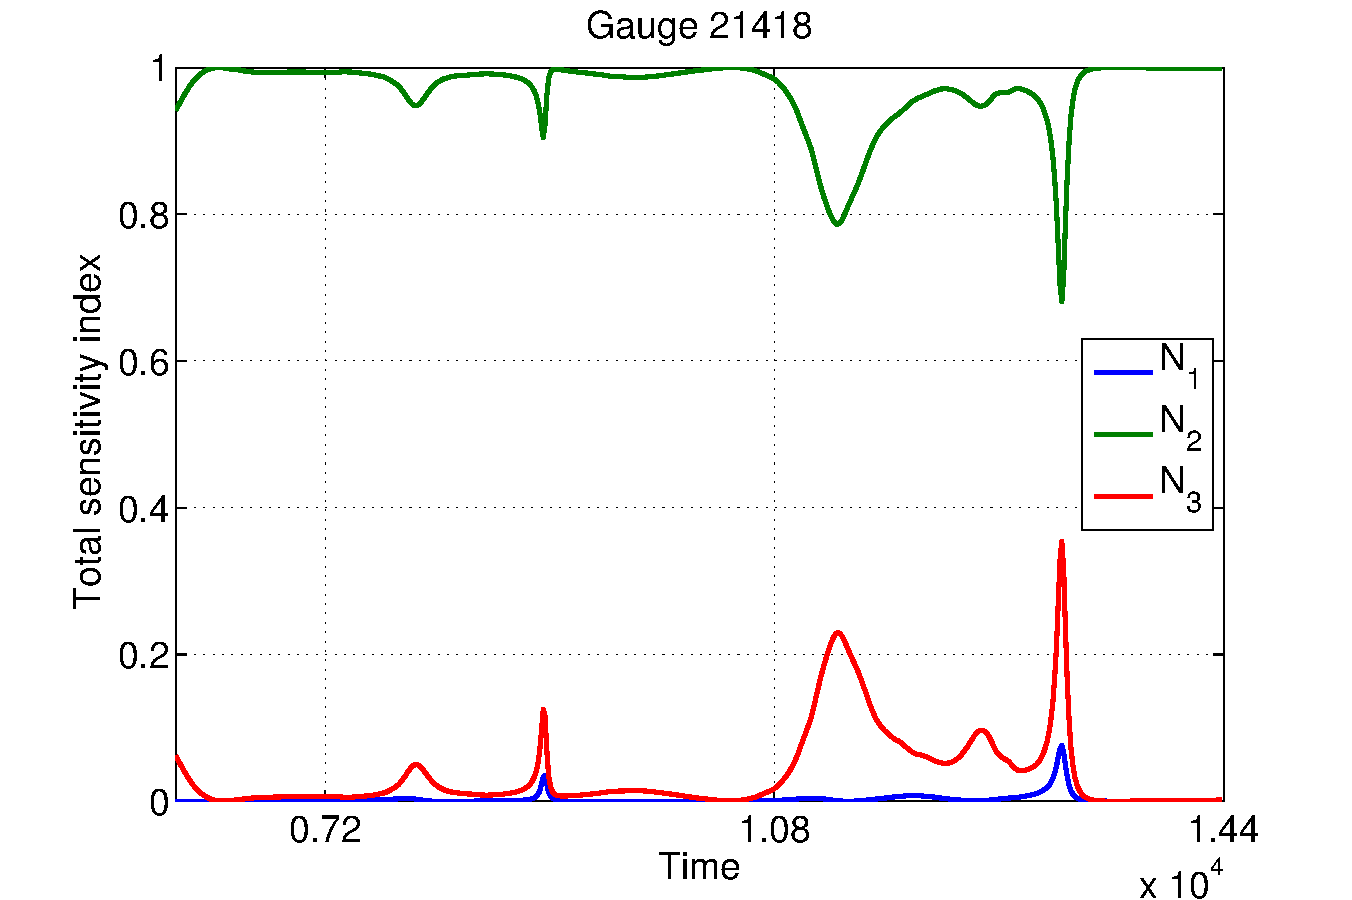
\includegraphics[width=0.475\textwidth]{./figures/sens3.pdf} &
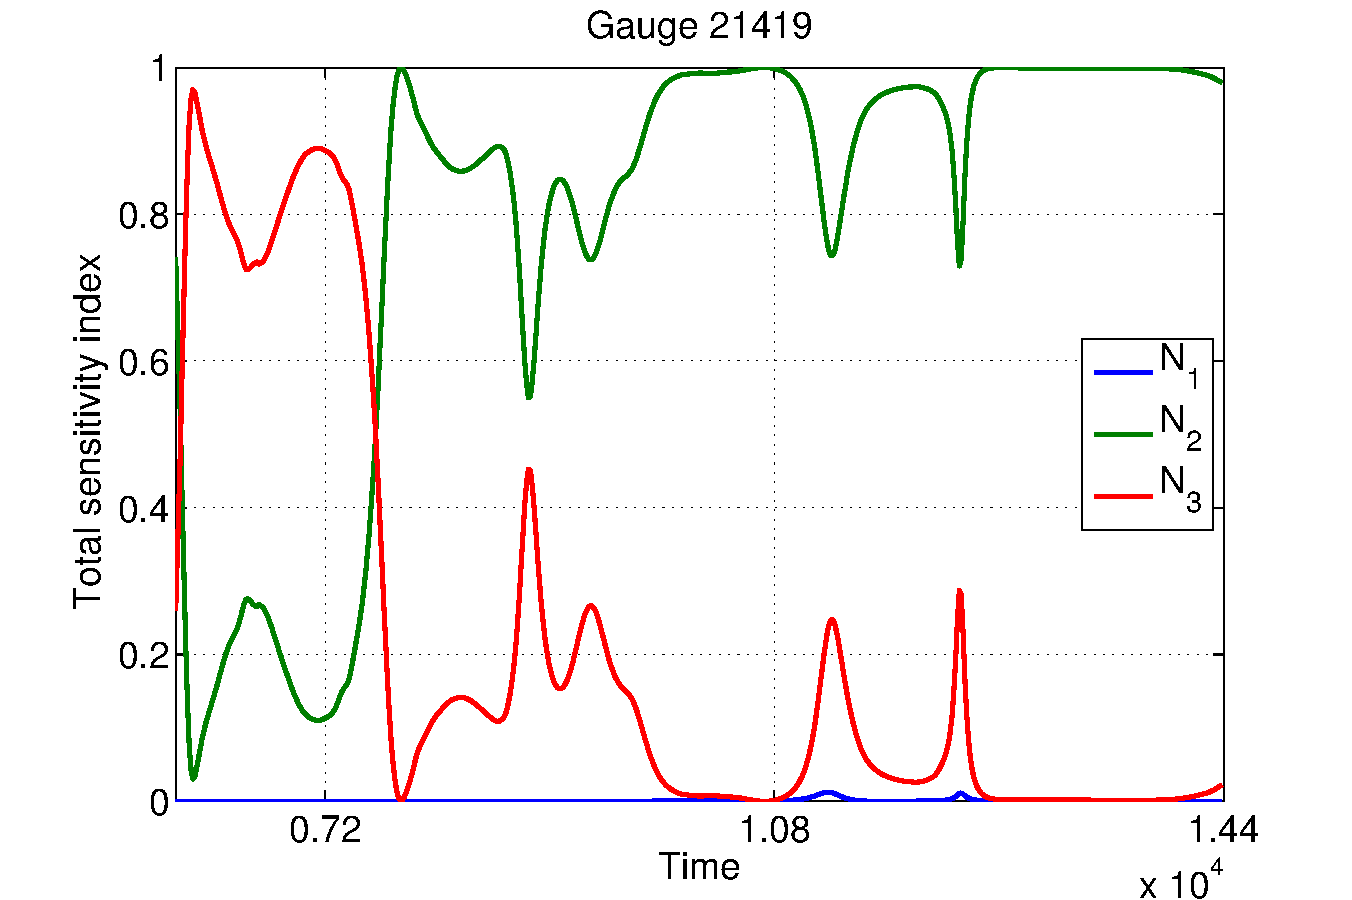
\includegraphics[width=0.475\textwidth]{./figures/sens4.pdf}
\end{tabular}
\caption{Total sensitivity index of different input parameters.}
\label{fig:sens}
\end{figure}

%%%%%%%%%%%%%%%%%%%%%%%%%%%%%%%%%%%%%%%%%%%%%%%%%%%%%%%%%%%%%%%%

\begin{figure}[h]
        \begin{tabular}{ccc}
\hspace*{-65pt}
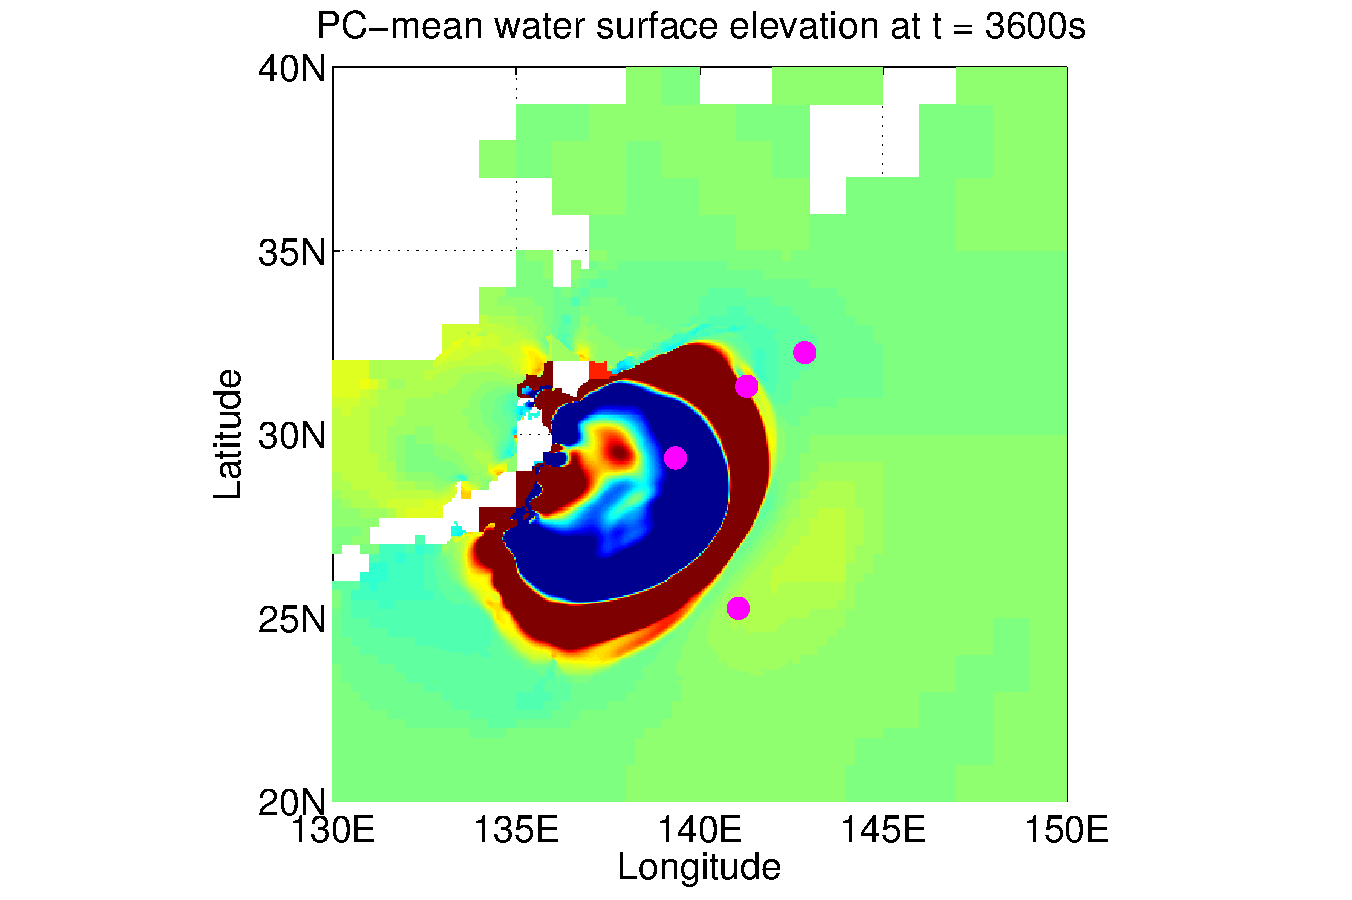
\includegraphics[width=0.45\textwidth]{./figures/mean2d1.pdf} &
\hspace*{-65pt}
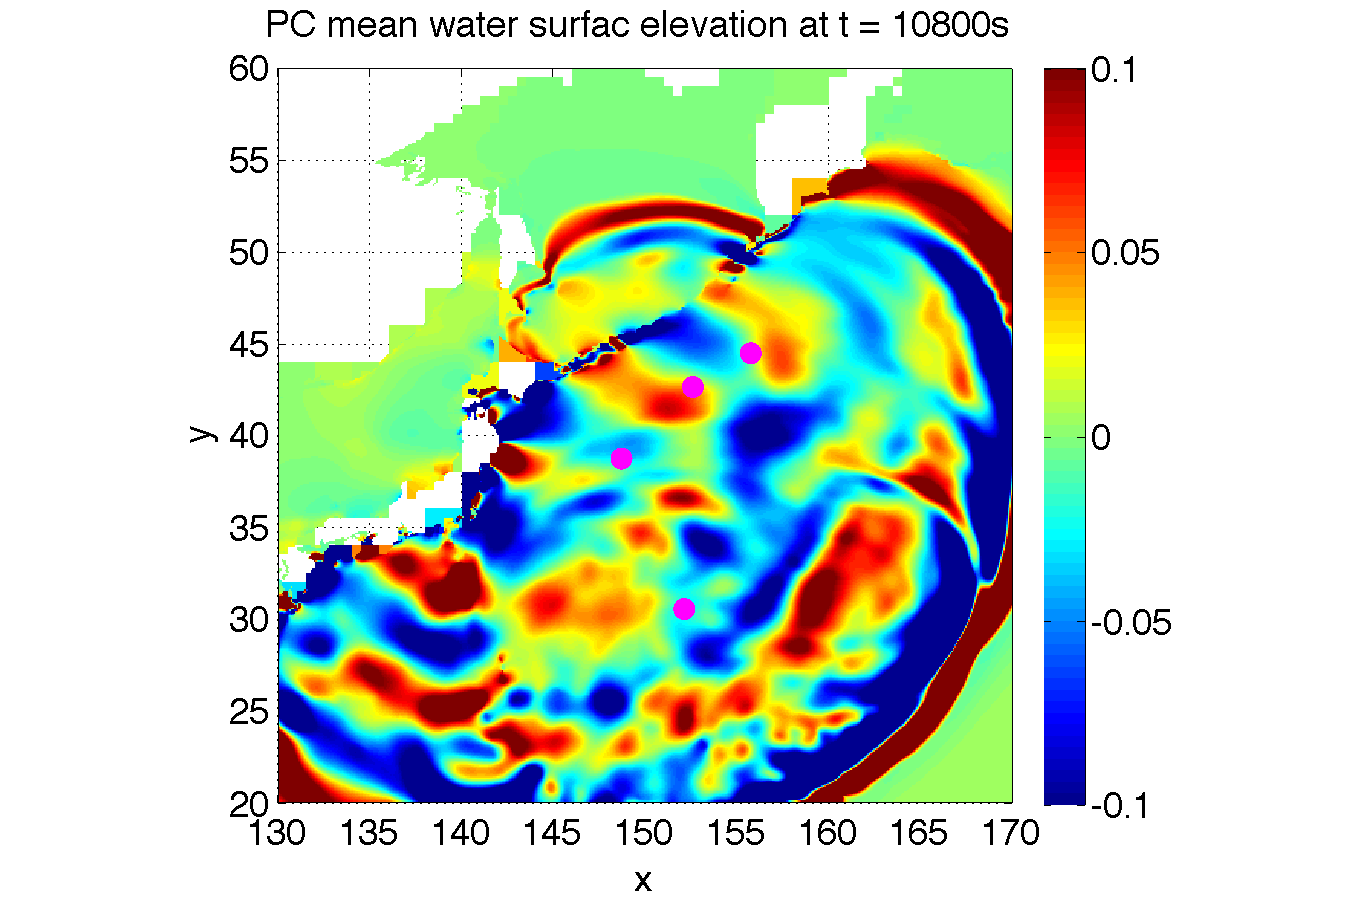
\includegraphics[width=0.45\textwidth]{./figures/mean2d3.pdf} &
\hspace*{-65pt}
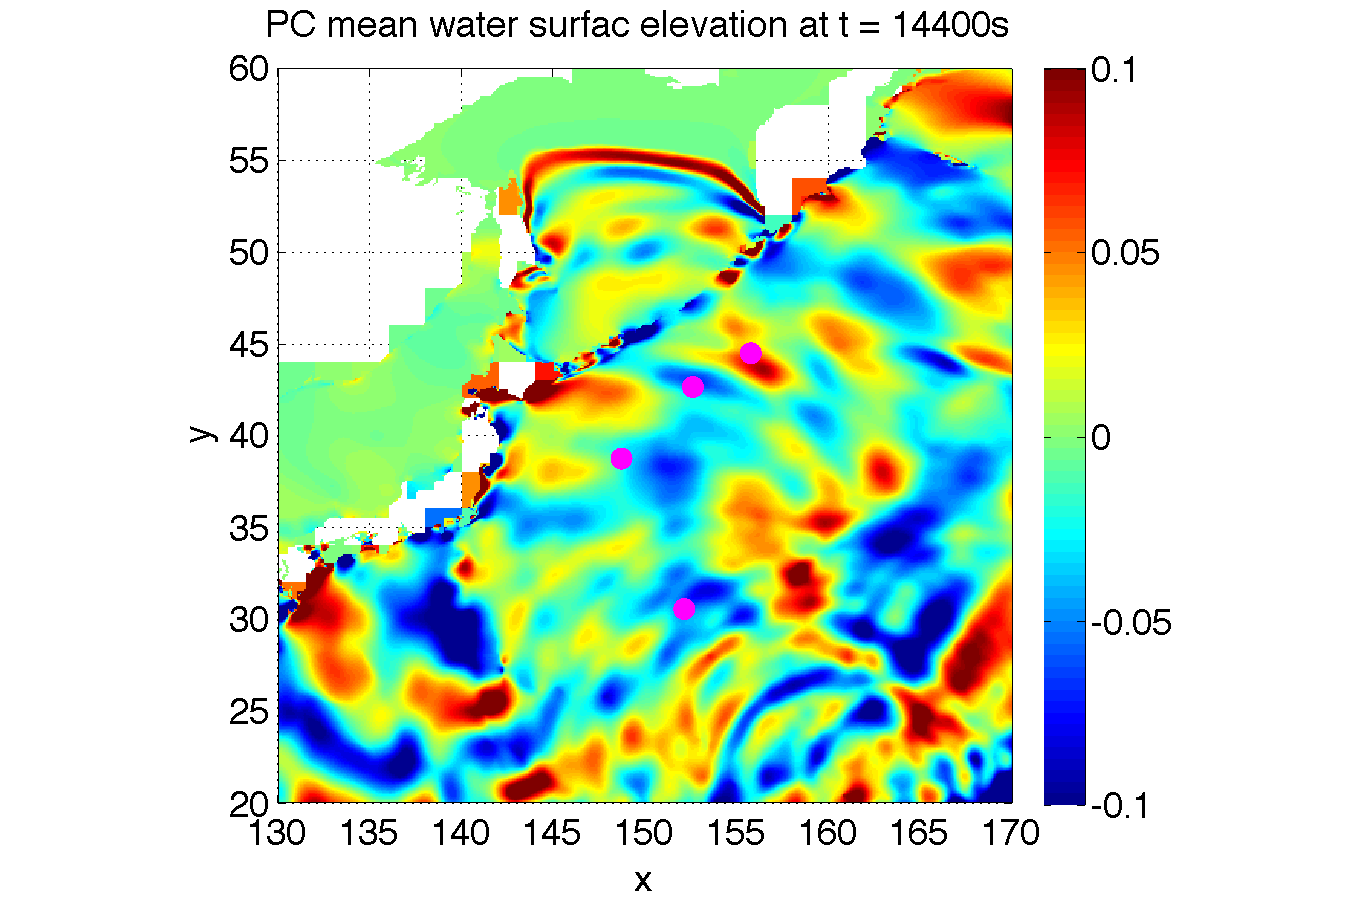
\includegraphics[width=0.45\textwidth]{./figures/mean2d4.pdf} \\
\hspace*{-65pt}
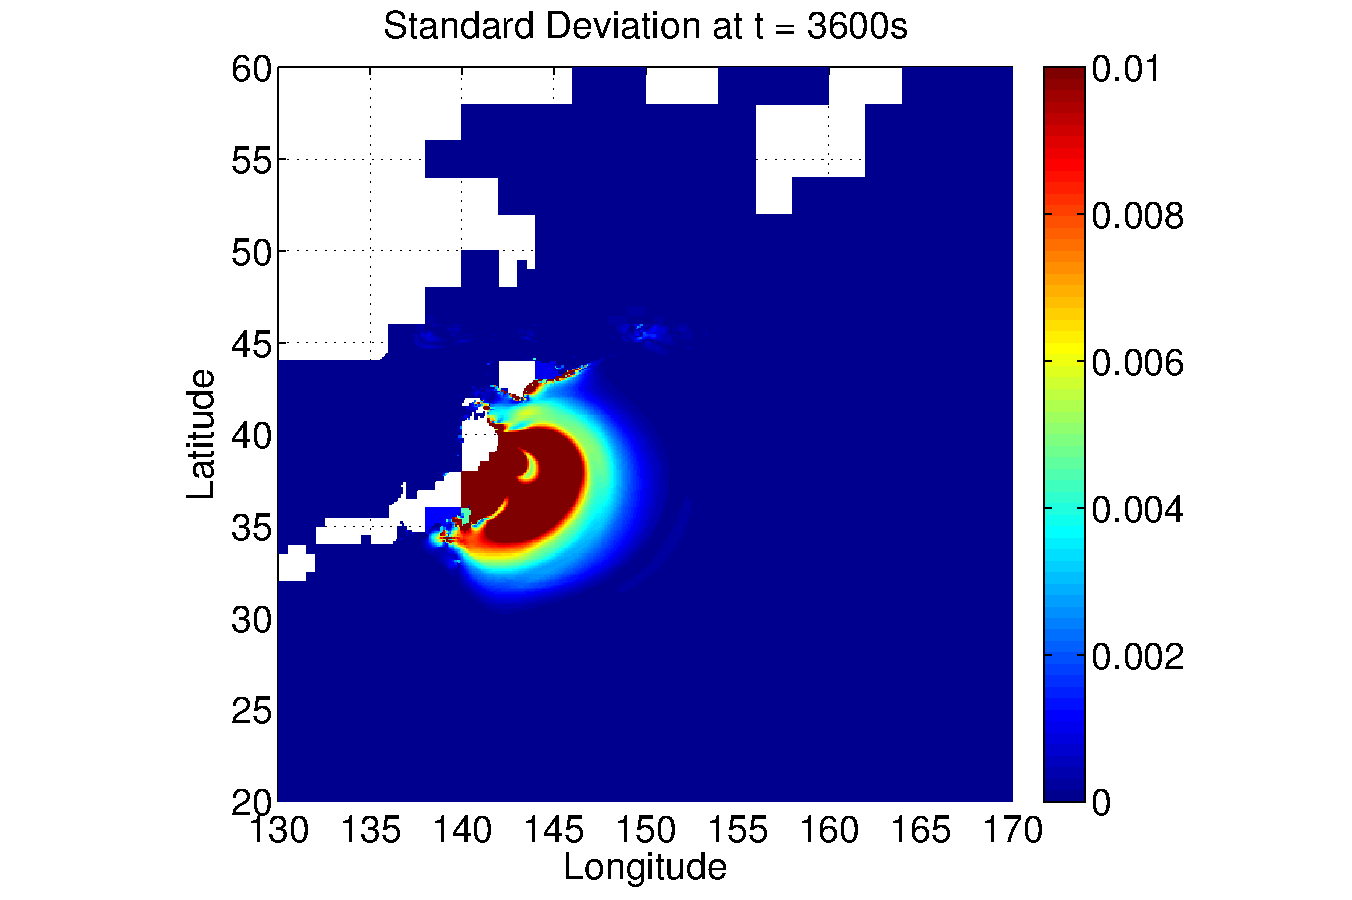
\includegraphics[width=0.45\textwidth]{./figures/sigma2d1.pdf} &
\hspace*{-65pt}
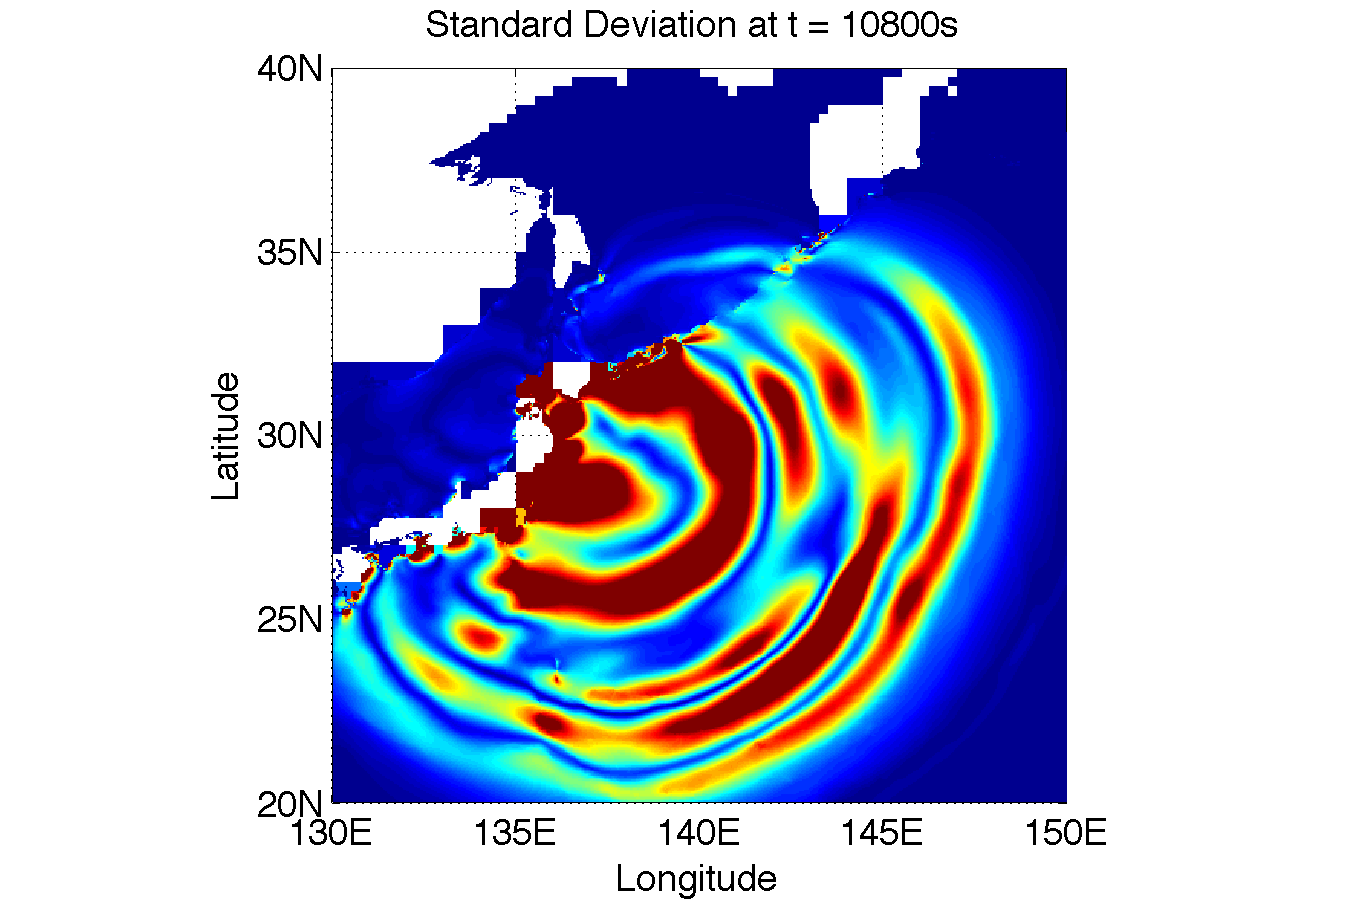
\includegraphics[width=0.45\textwidth]{./figures/sigma2d3.pdf} &
\hspace*{-65pt}
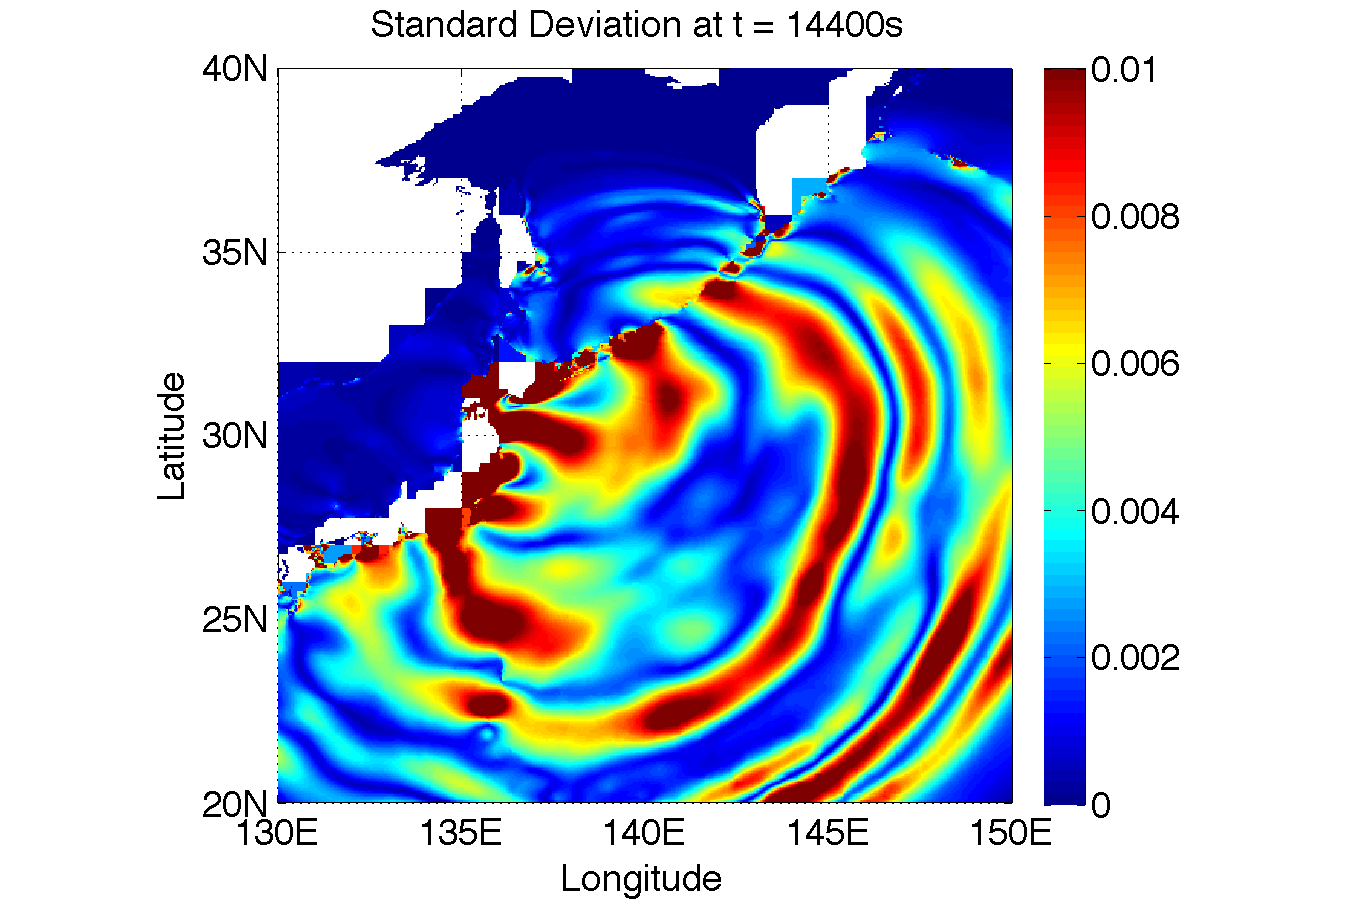
\includegraphics[width=0.45\textwidth]{./figures/sigma2d4.pdf}
\end{tabular}
\caption{PC mean (top row) and standard deviation (bottom row) of the water surface elevation at different times.}
\label{fig:mean2d}
\end{figure}
      %%%%%%%%%%%%%%%%%%%%%%%%%%%%%%%%%%%%%%%%%%%%%%%%%%%%%%%%%%%%%%%%

\begin{figure}[h]
\begin{tabular}{clc}
 \hspace*{-65pt}
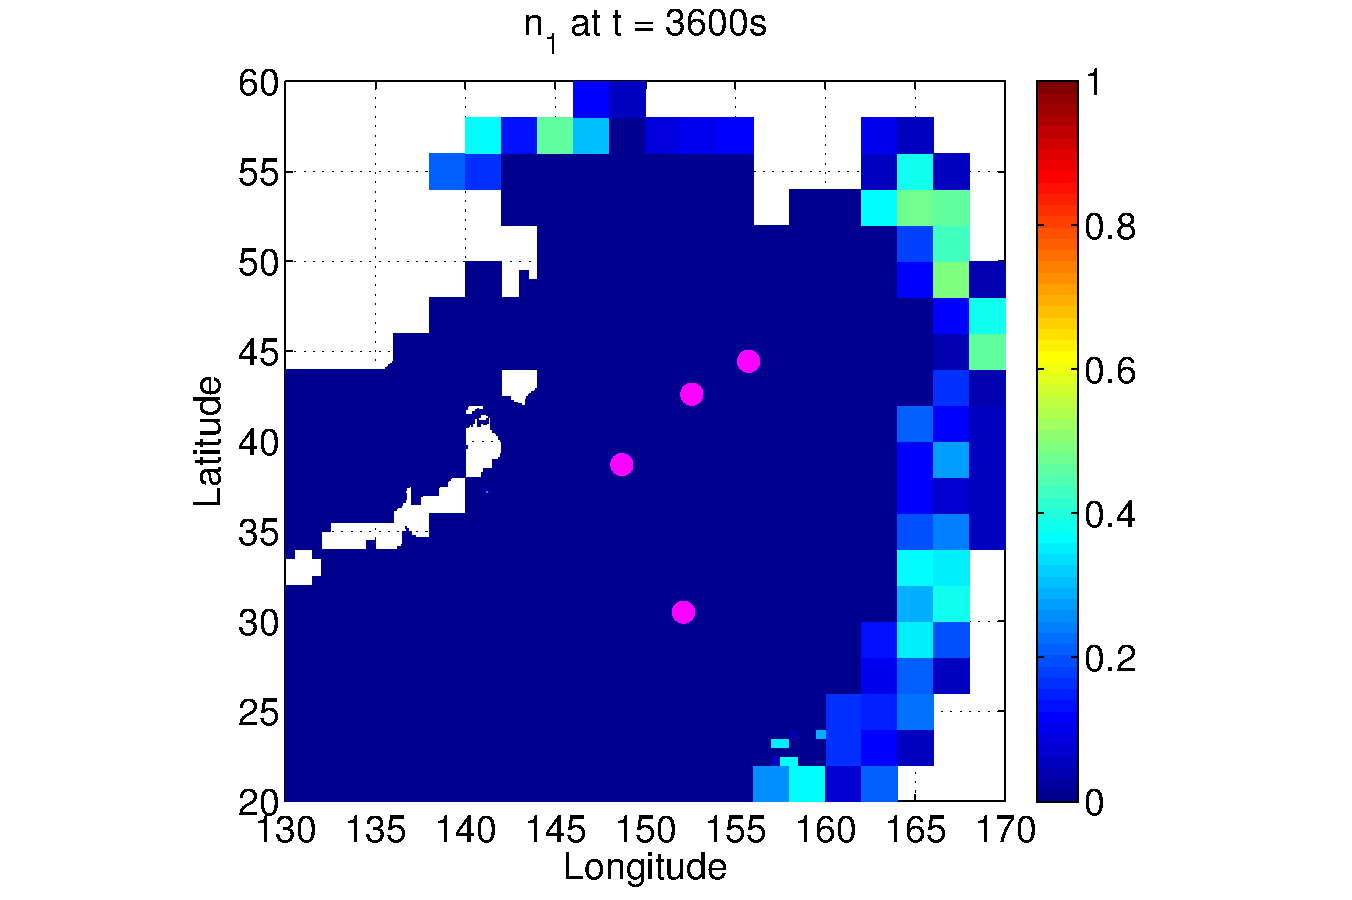
\includegraphics[width=0.45\textwidth]{./figures/T12d1.pdf} &
\hspace*{-65pt}
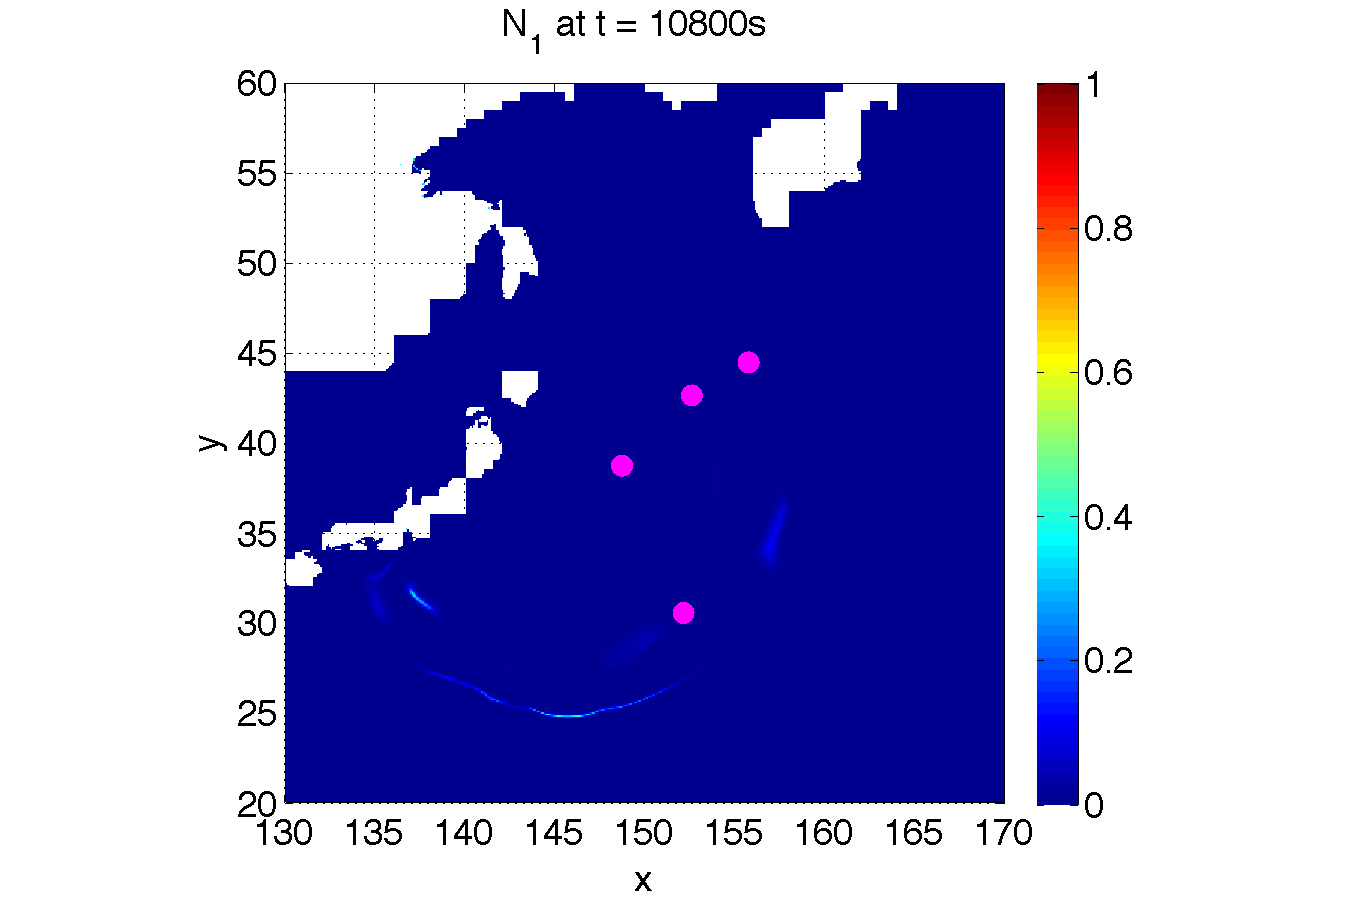
\includegraphics[width=0.45\textwidth]{./figures/T12d3.pdf} &
\hspace*{-65pt}
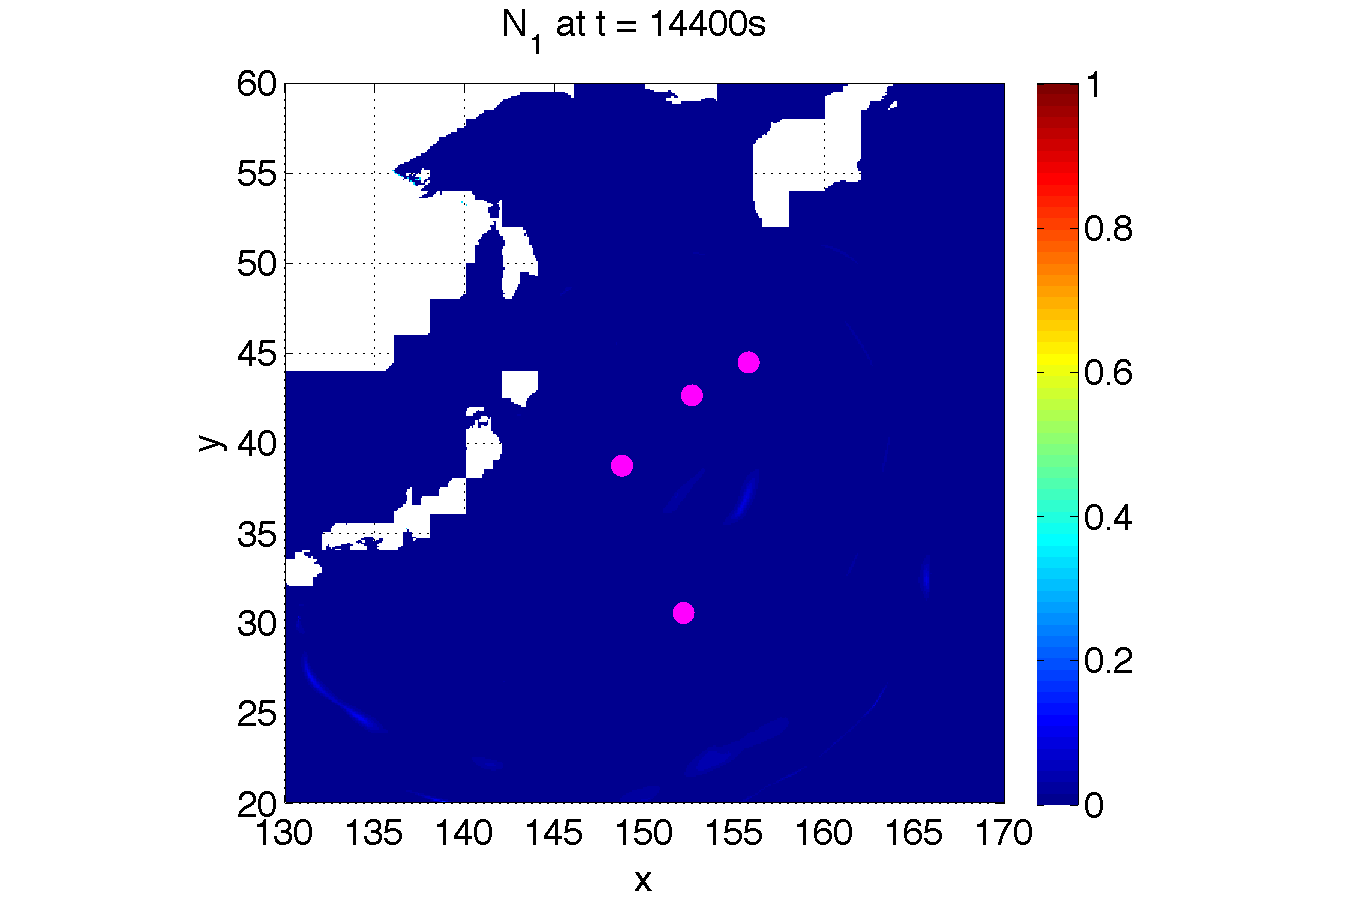
\includegraphics[width=0.45\textwidth]{./figures/T12d4.pdf} \\
\hspace*{-65pt}
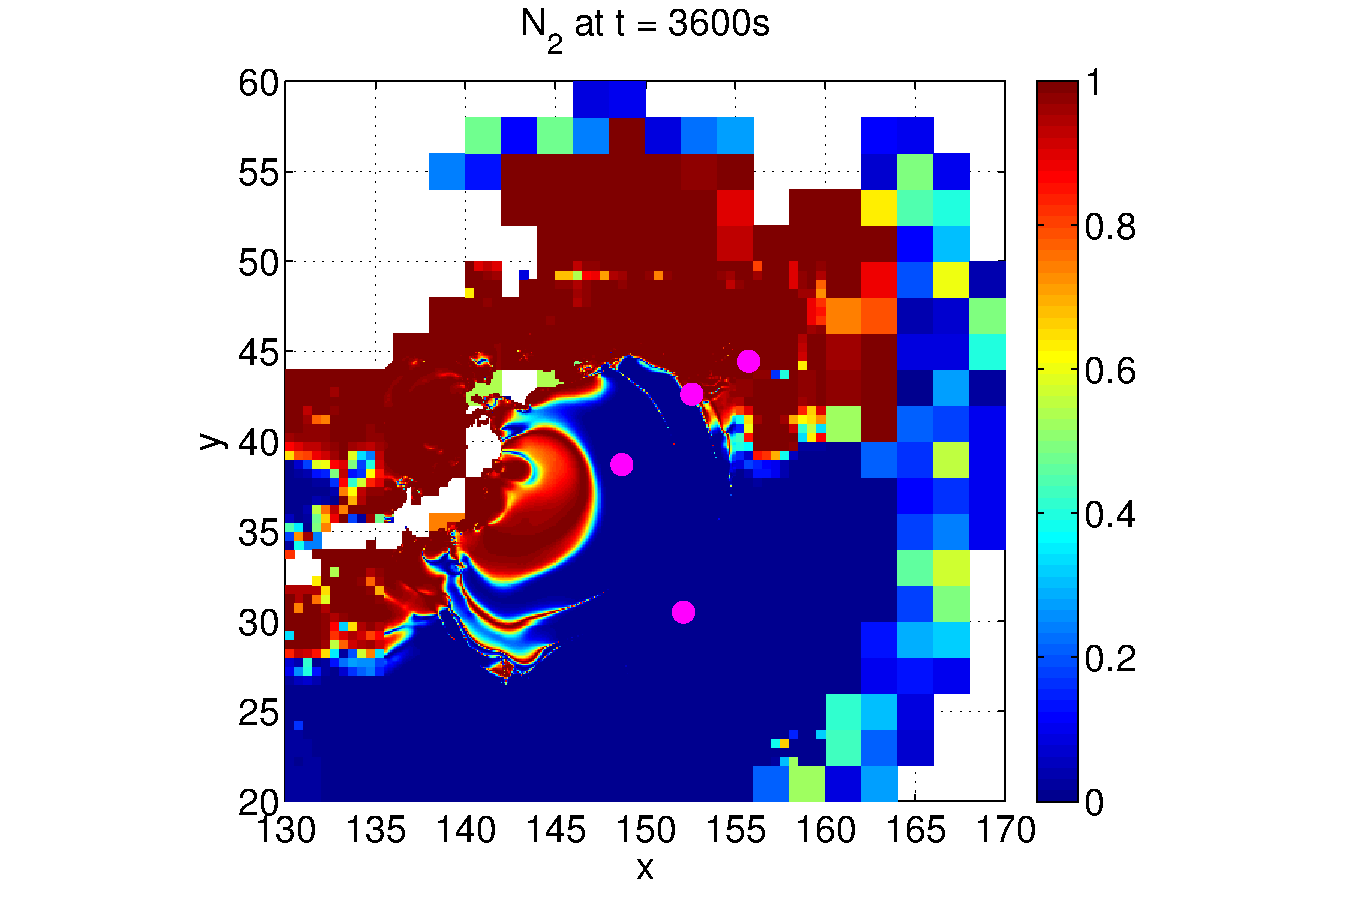
\includegraphics[width=0.45\textwidth]{./figures/T22d1.pdf} &
\hspace*{-65pt}
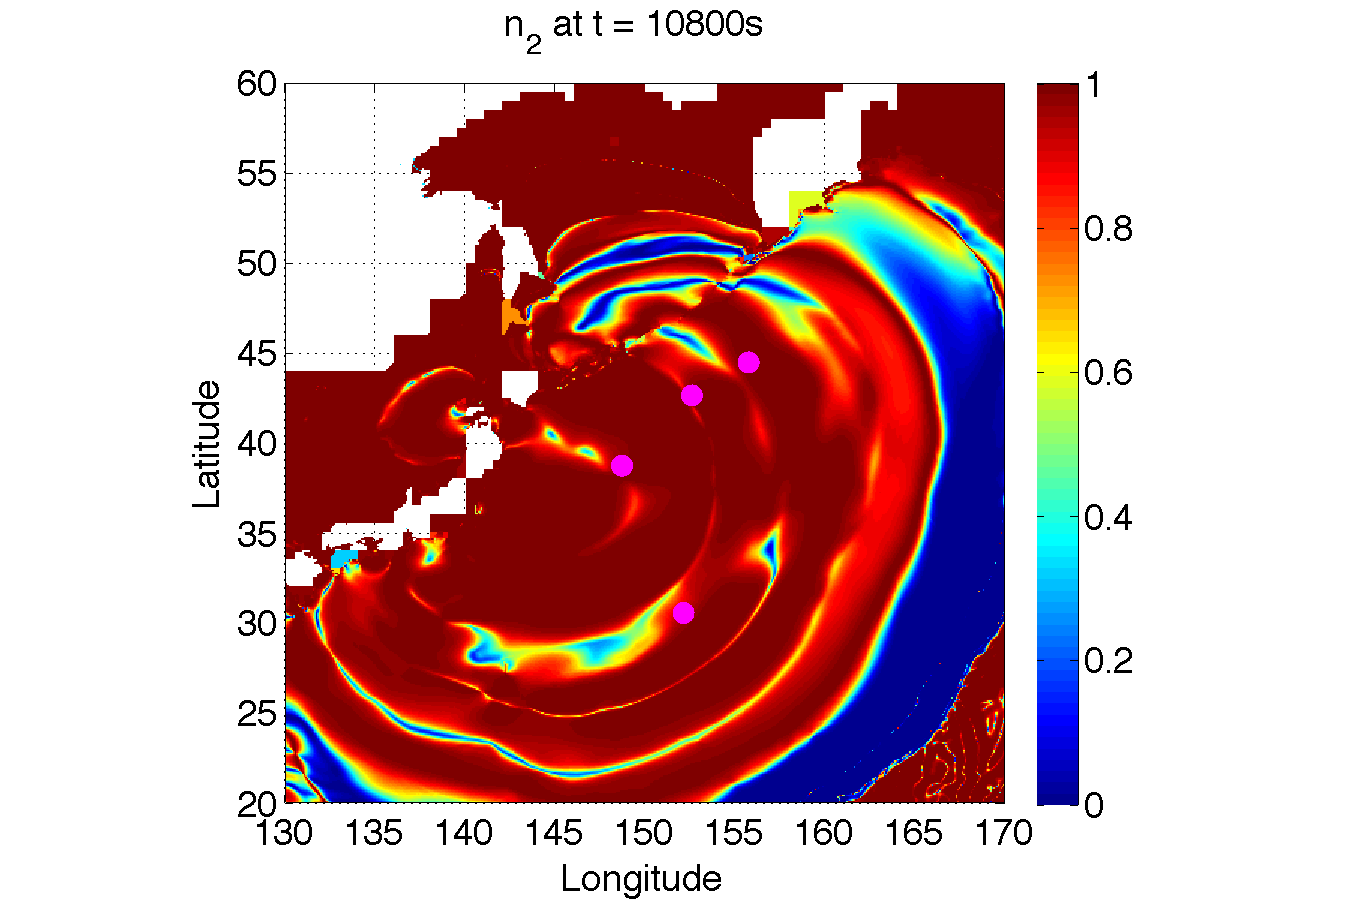
\includegraphics[width=0.45\textwidth]{./figures/T22d3.pdf} &
\hspace*{-65pt}
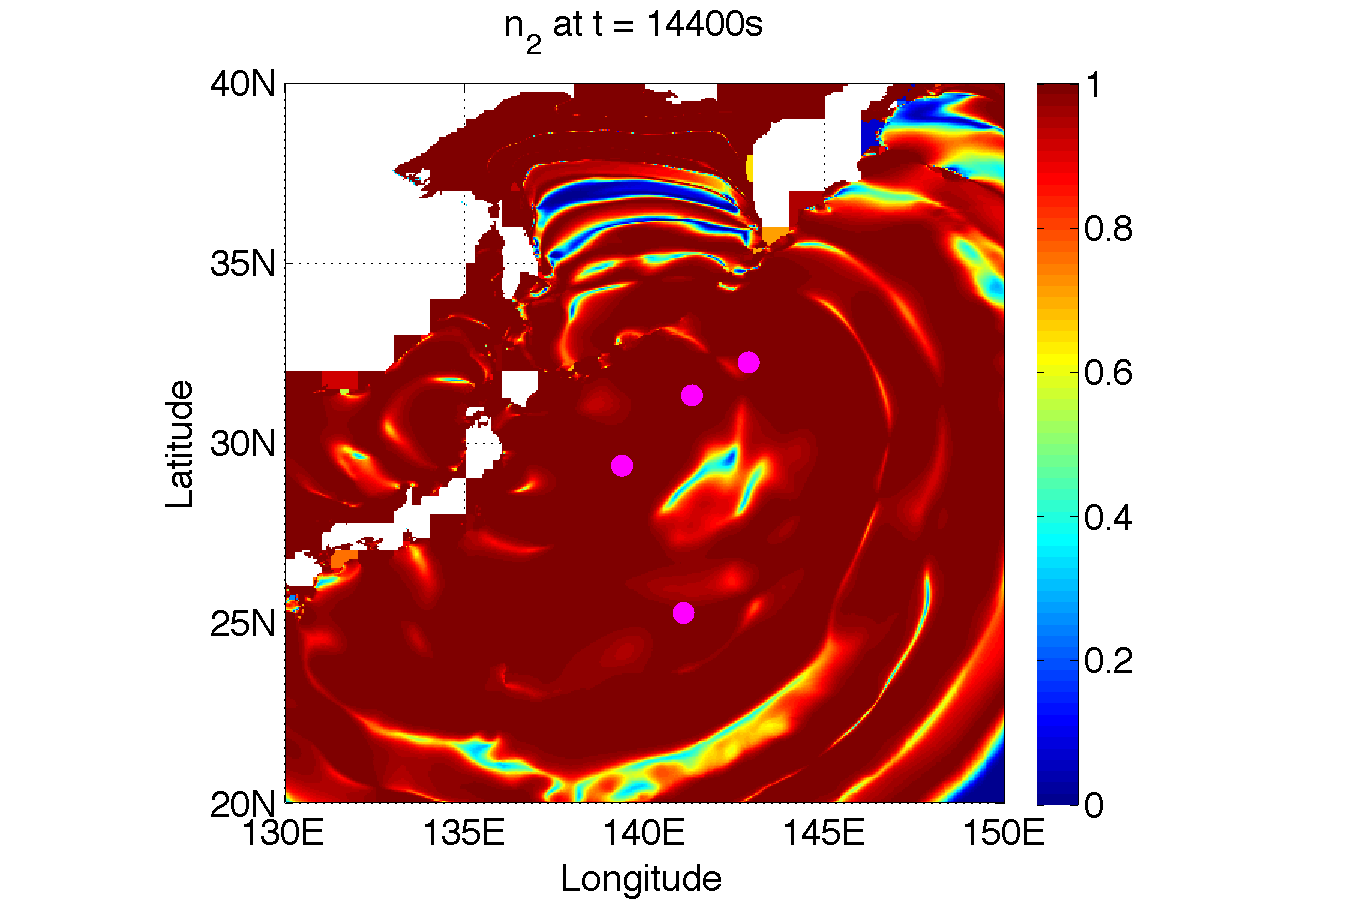
\includegraphics[width=0.45\textwidth]{./figures/T22d4.pdf} \\
\hspace*{-65pt}
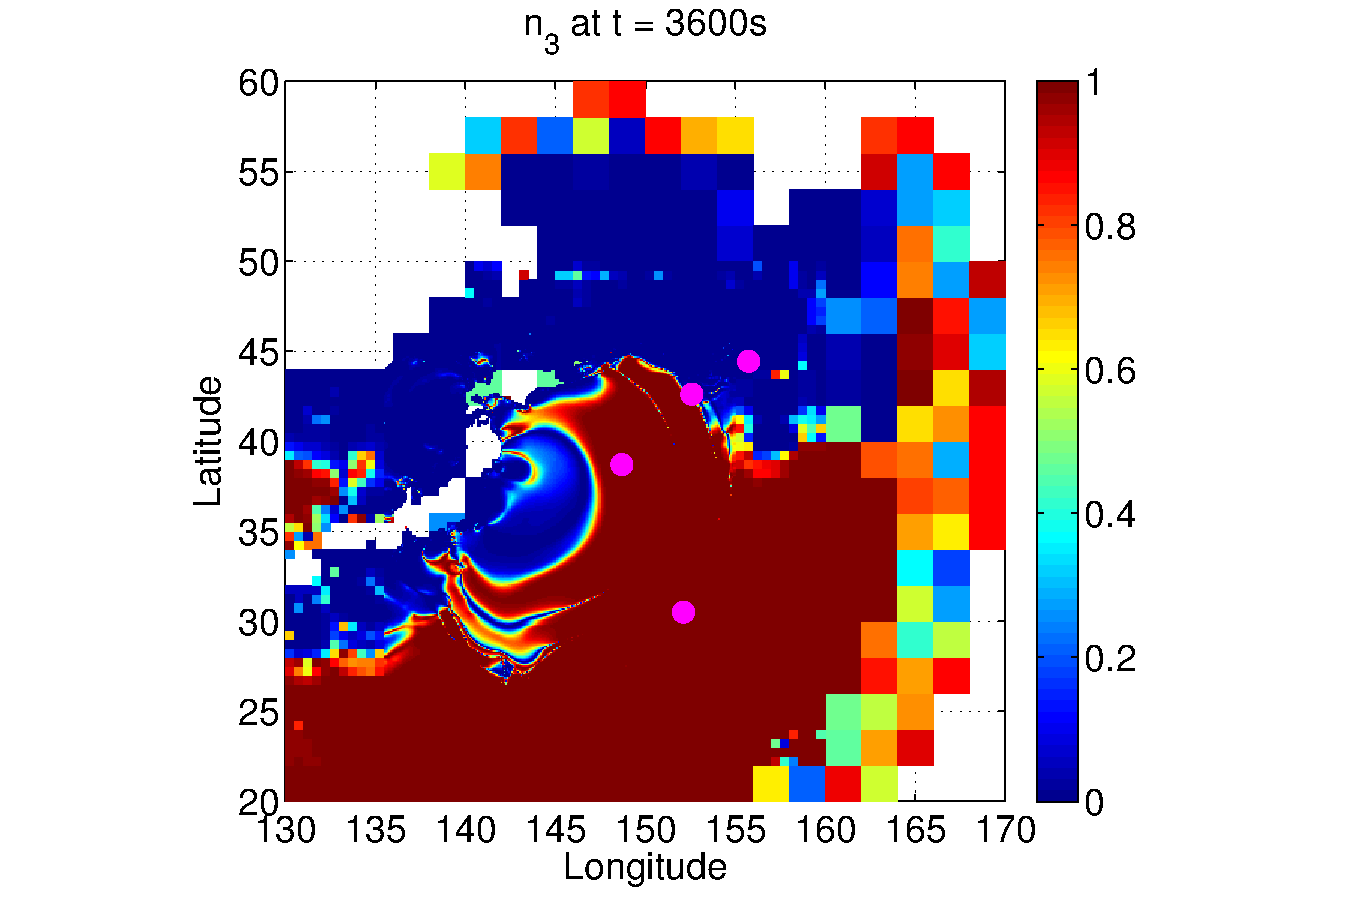
\includegraphics[width=0.45\textwidth]{./figures/T32d1.pdf} &
\hspace*{-65pt}
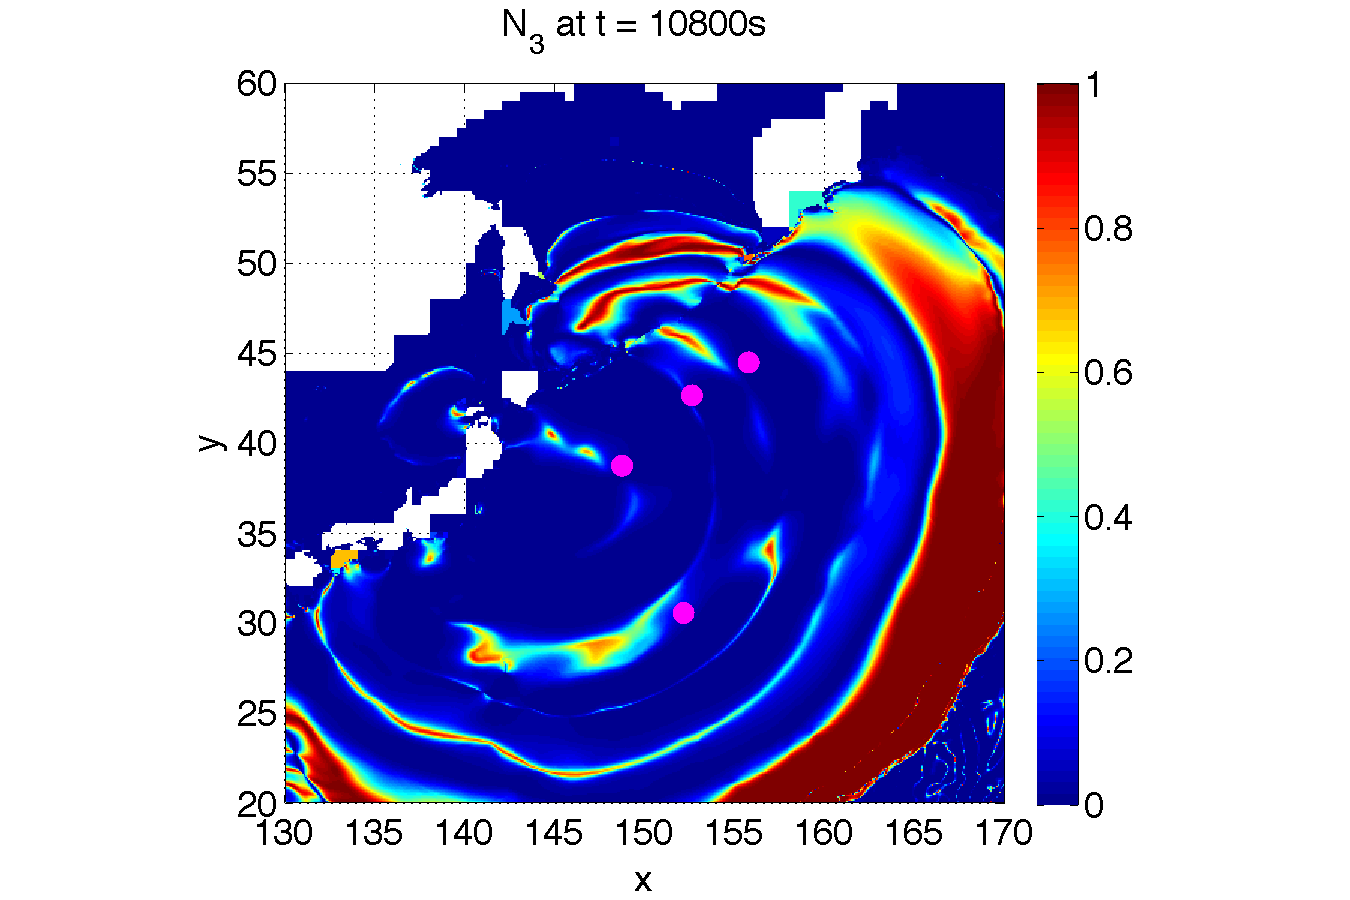
\includegraphics[width=0.45\textwidth]{./figures/T32d3.pdf} &
\hspace*{-65pt}
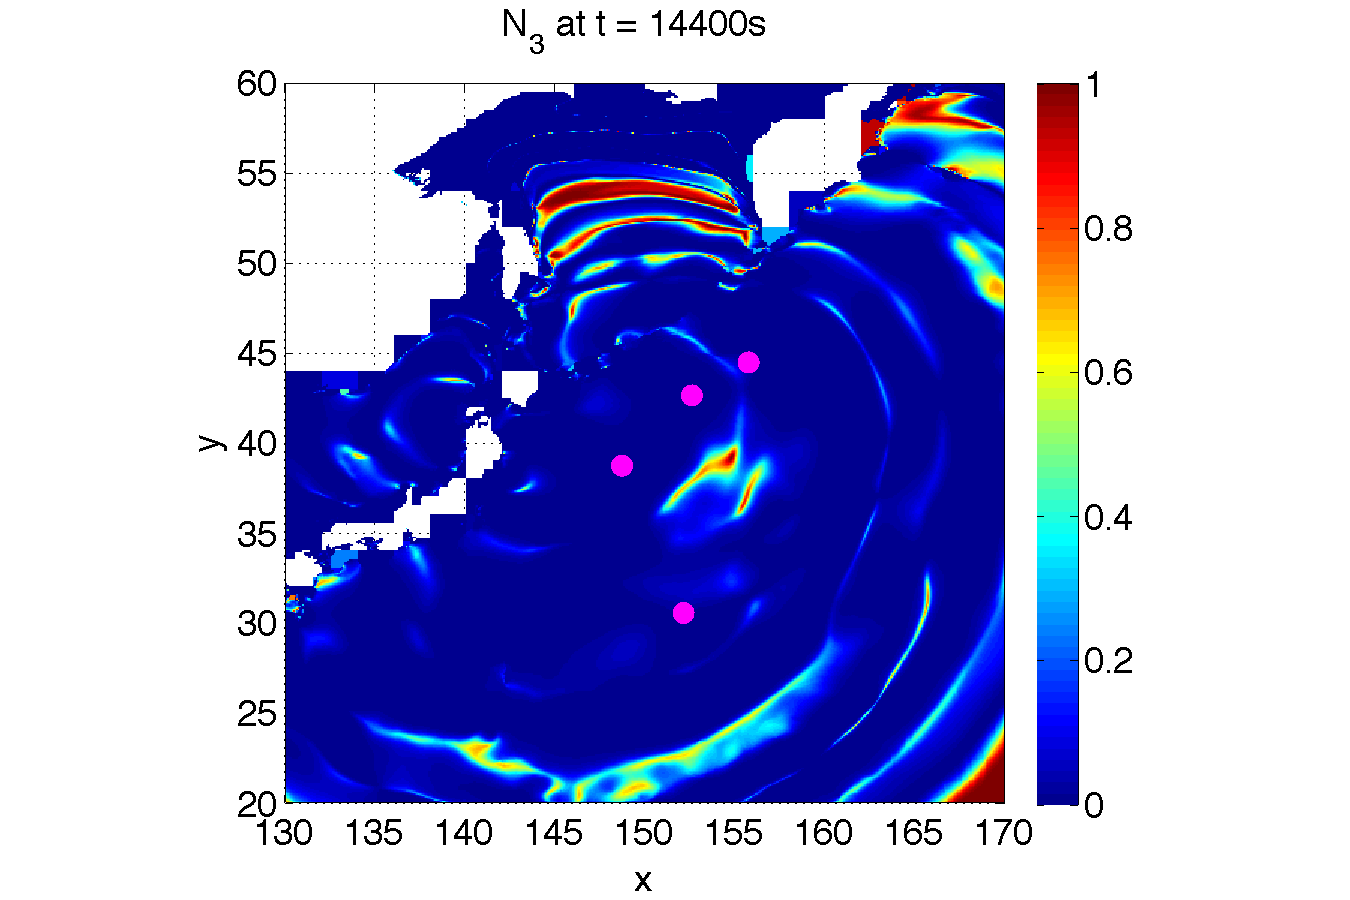
\includegraphics[width=0.45\textwidth]{./figures/T32d4.pdf}
\end{tabular}
\caption{Total sensitivity index for $N_1$ (top row) $N_2$ (center row) and $N_3$ (bottom row)
 at different times as indicated.}
\label{fig:sens2d}
\end{figure}
%%%%%%%%%%%%%%%%%%%%%%%%%%%%%%%%%%%%%%%%%%%%%%%%%%%%%%%%%%%%%%%%
\begin{figure}[h]
\centering

\begin{tabular}{clcl}
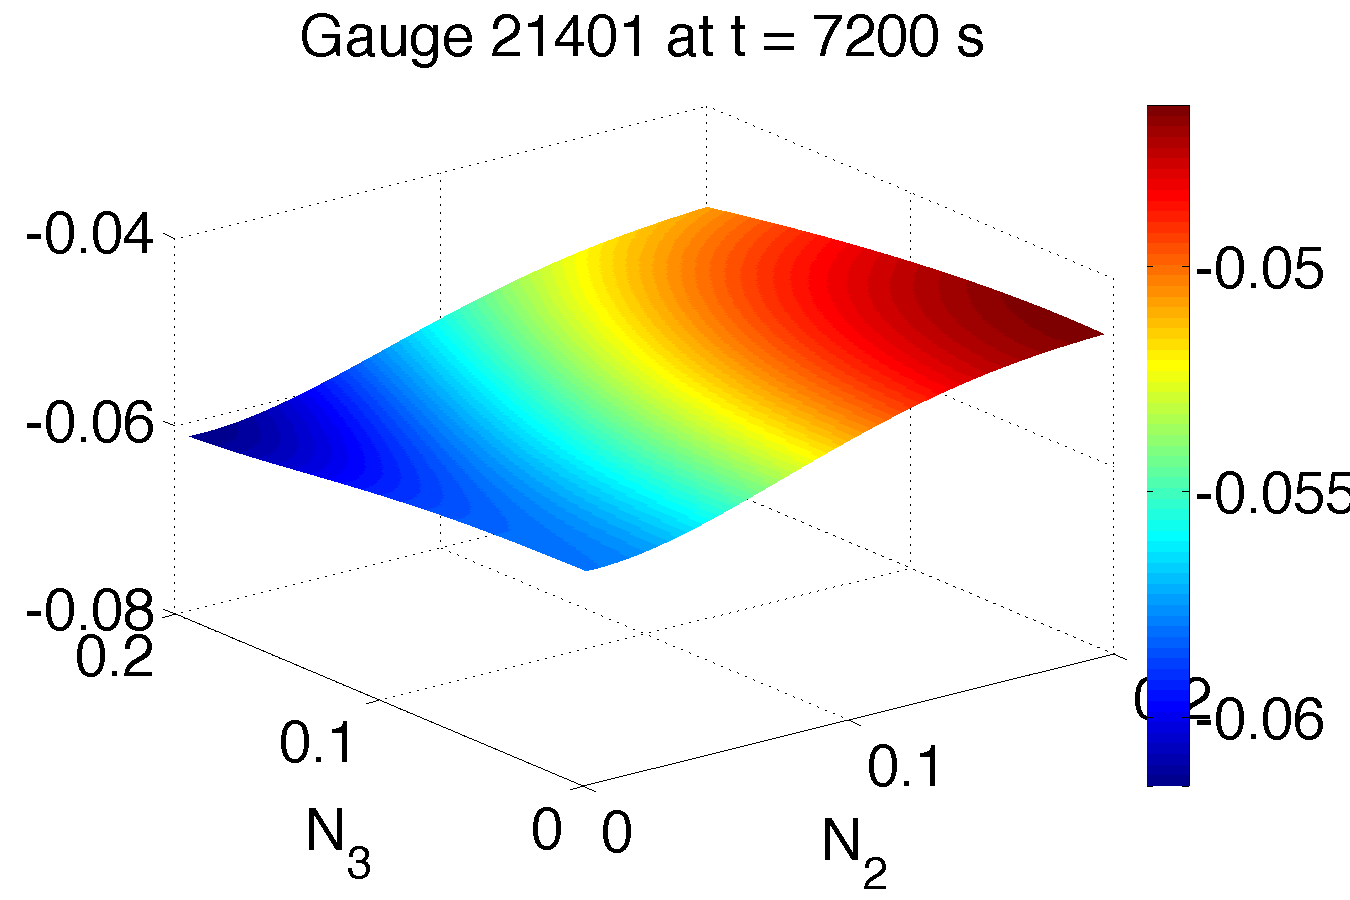
\includegraphics[width=0.5\textwidth]{./figures/response_i1_t2.pdf} &
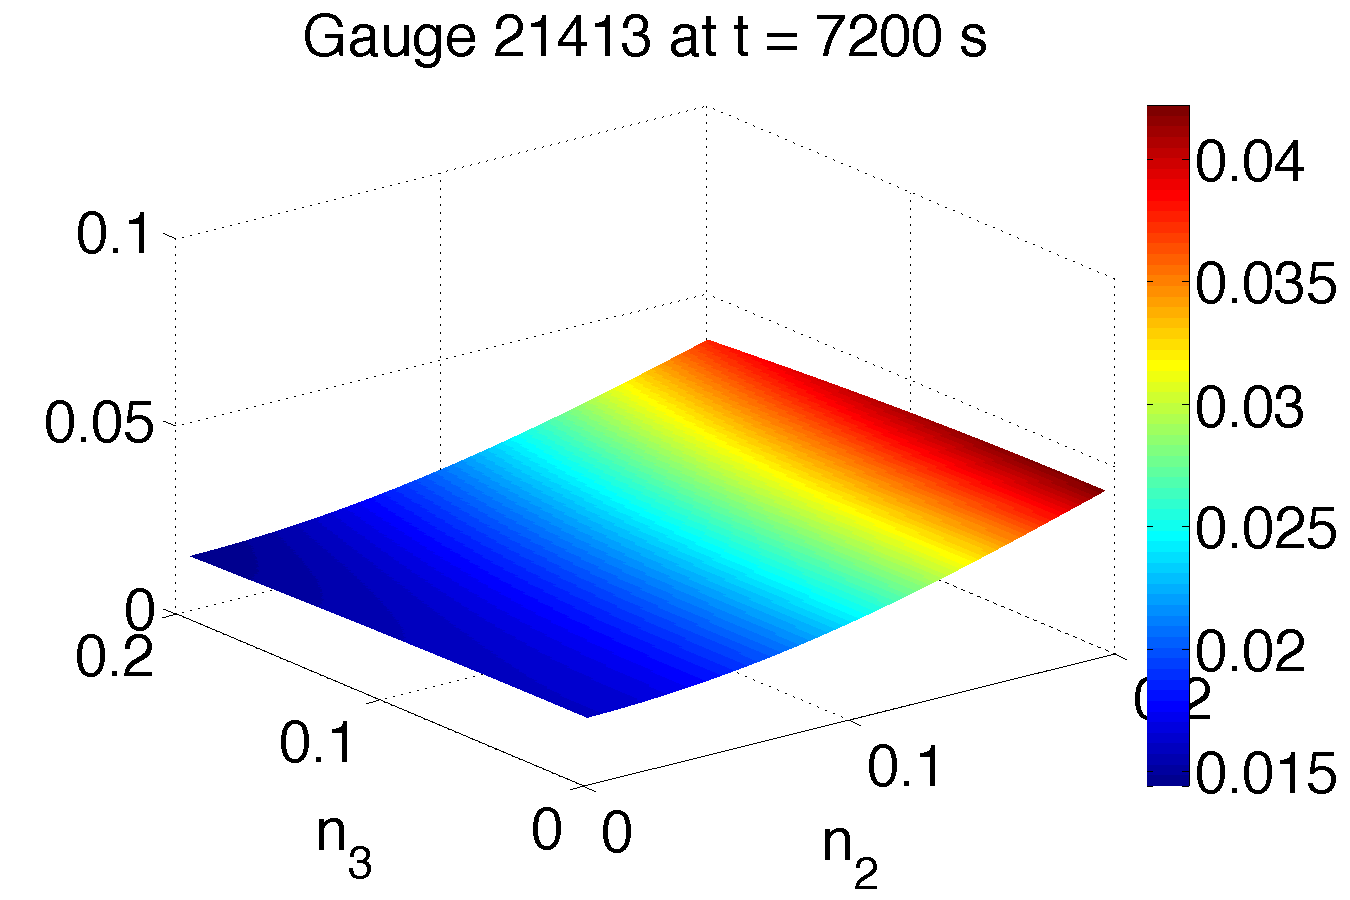
\includegraphics[width=0.5\textwidth]{./figures/response_i2_t2.pdf} \\
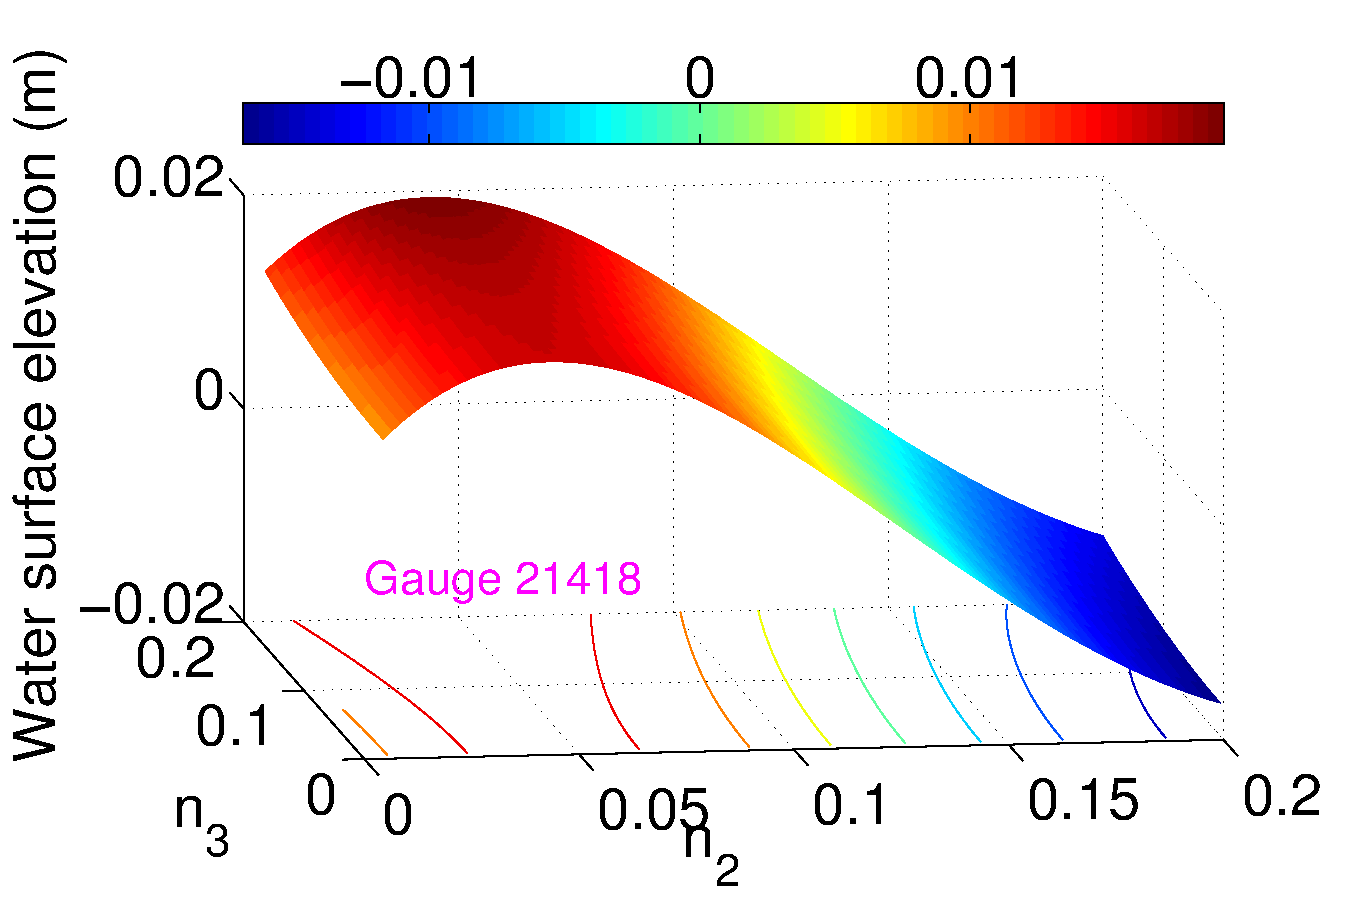
\includegraphics[width=0.5\textwidth]{./figures/response_i3_t2.pdf} &
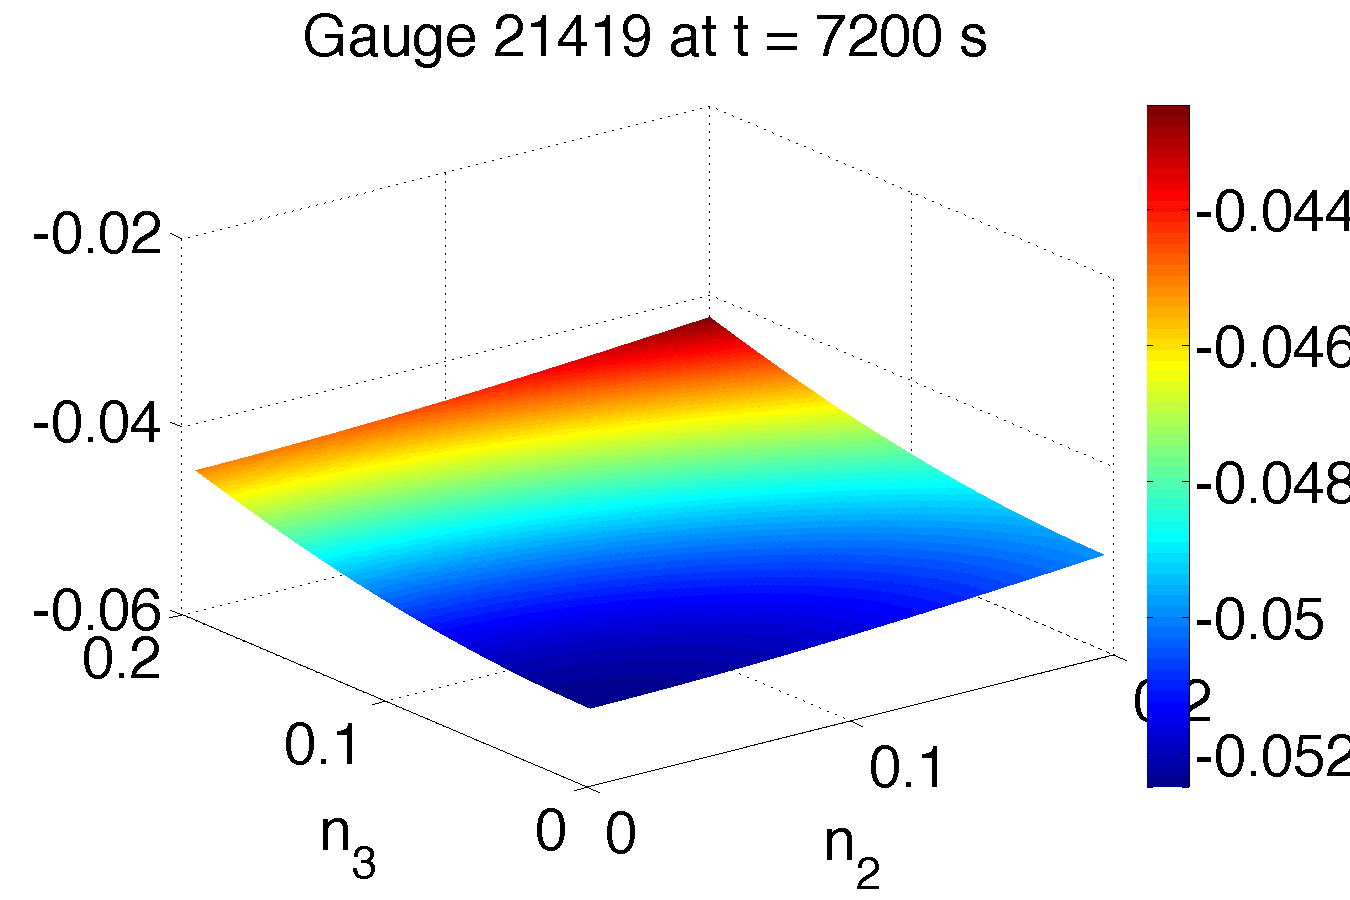
\includegraphics[width=0.5\textwidth]{./figures/response_i4_t2.pdf}
\end{tabular}
\caption{Response surface of water surface elevation at the different gauge locations at t = 7200 s.}
\label{fig:response2}
\end{figure}
%%%%%%%%%%%%%%%%%%%%%%%%%%%%%%%%%%%%%%%%%%%%%%%%%%%%%%%%%%%%%%%%
\begin{figure}[h]
\centering

\begin{tabular}{clcl}
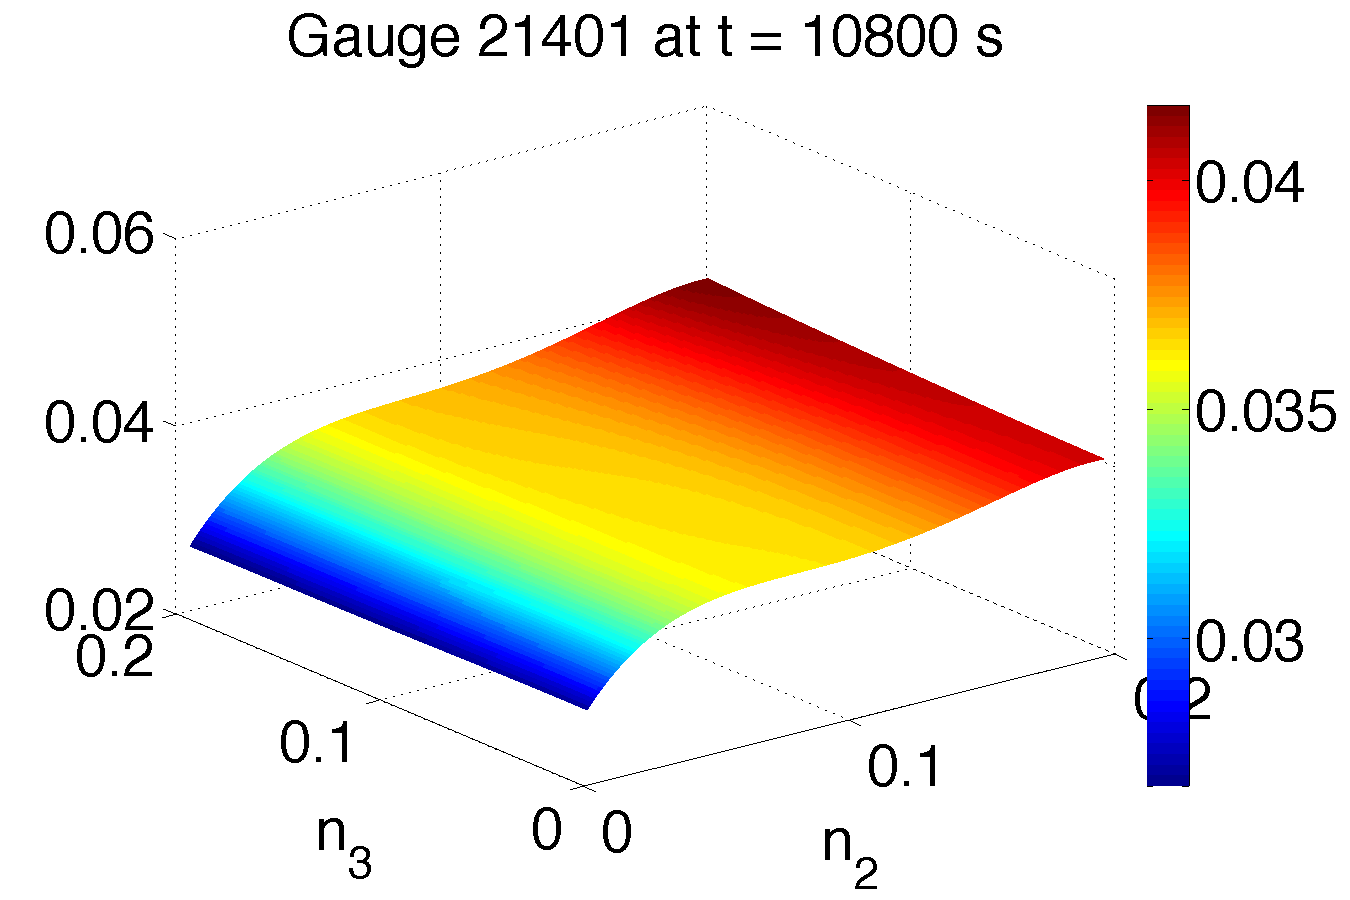
\includegraphics[width=0.5\textwidth]{./figures/response_i1_t3.pdf} &
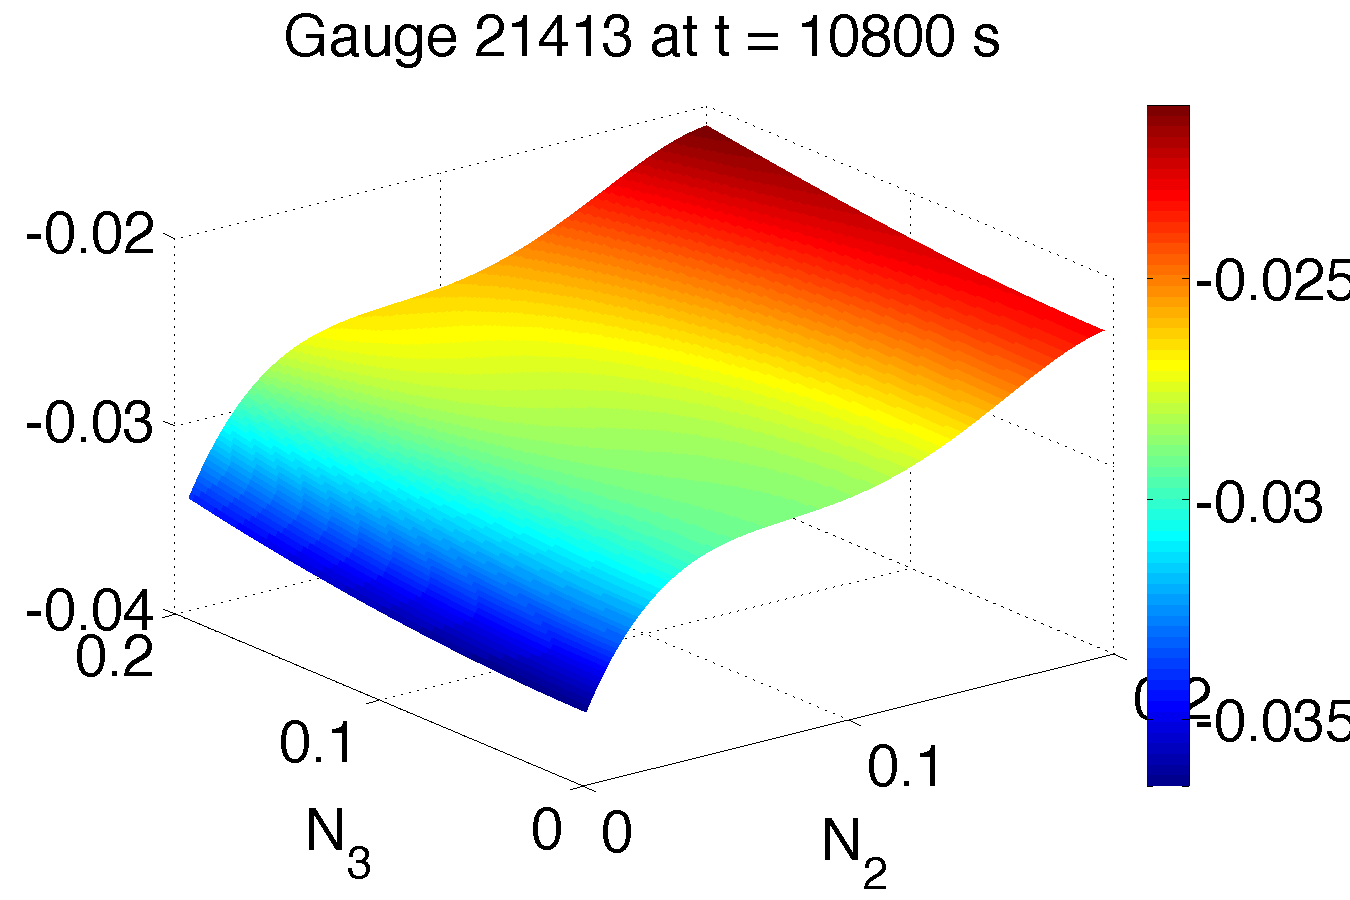
\includegraphics[width=0.5\textwidth]{./figures/response_i2_t3.pdf} \\
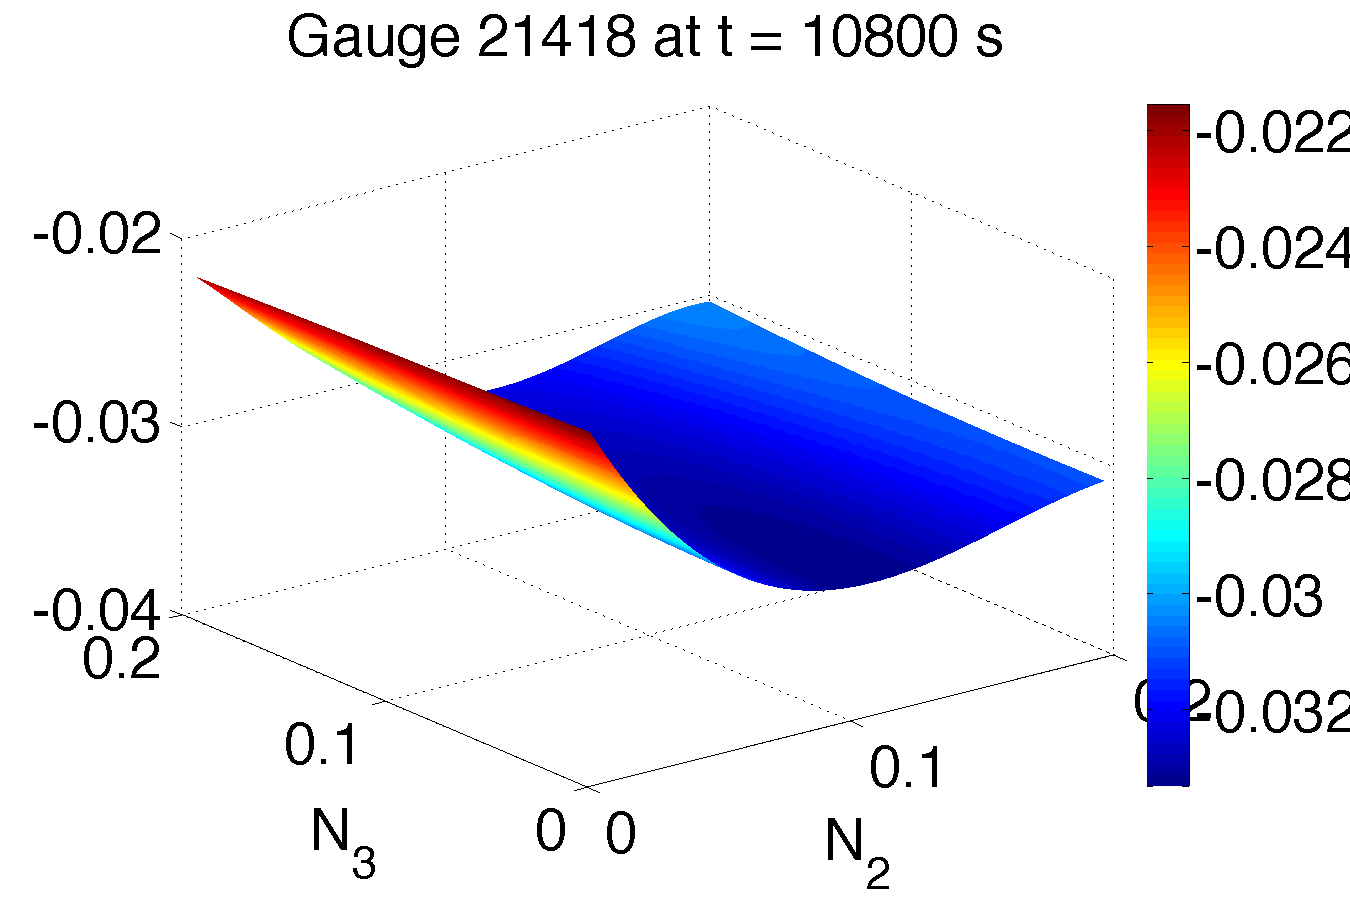
\includegraphics[width=0.5\textwidth]{./figures/response_i3_t3.pdf} &
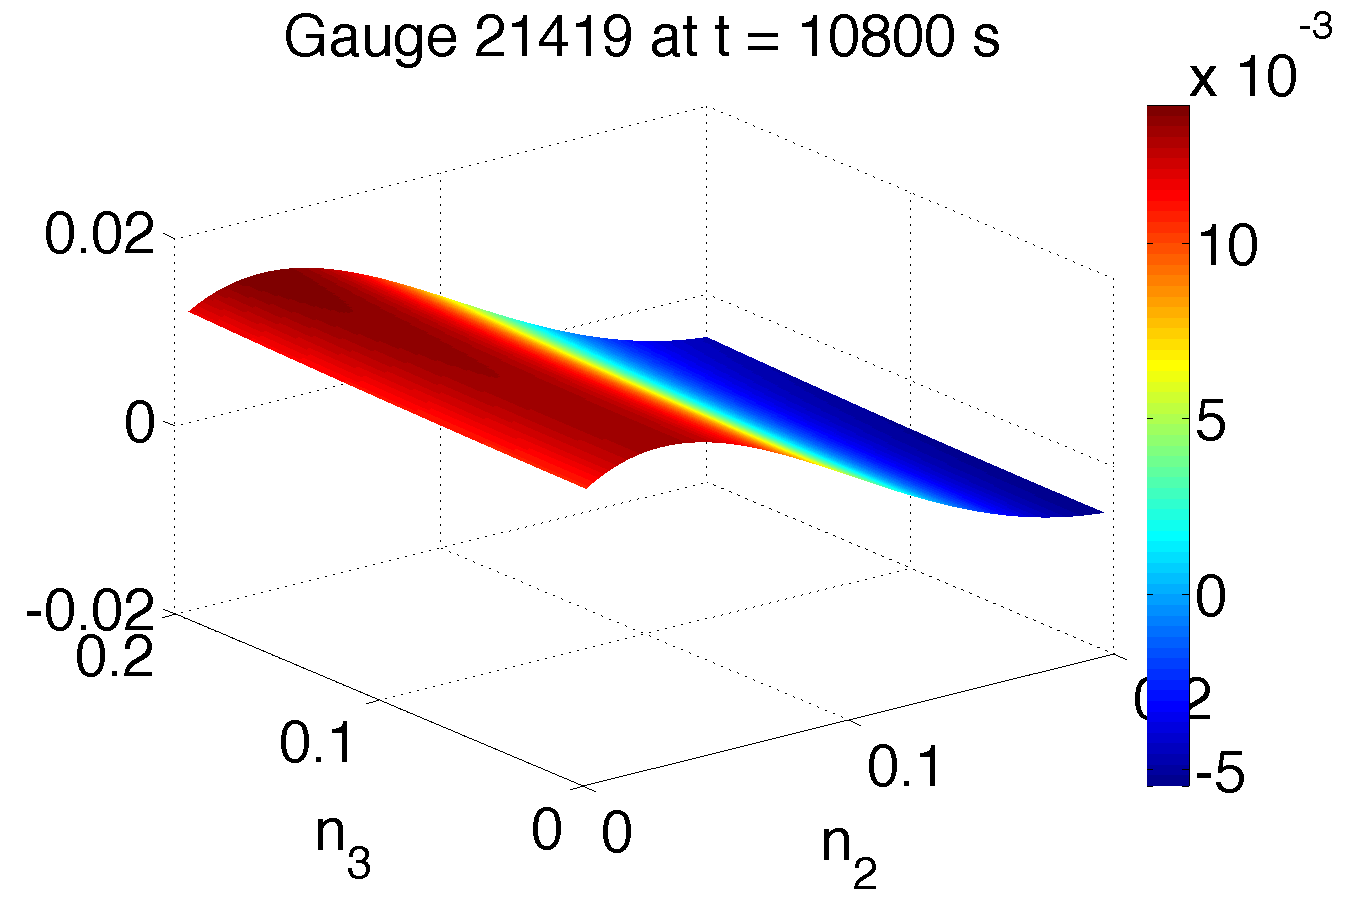
\includegraphics[width=0.5\textwidth]{./figures/response_i4_t3.pdf}
\end{tabular}
\caption{Response surface of water surface elevation at the different gauge locations at t = 14400 s.}
\label{fig:response3}
\end{figure}
%%%%%%%%%%%%%%%%%%%%%%%%%%%%%%%%%%%%%%%%%%%%%%%%%%%%%%%%%%%%%%%%

\begin{figure}[h]
\begin{tabular}{clc}
%        
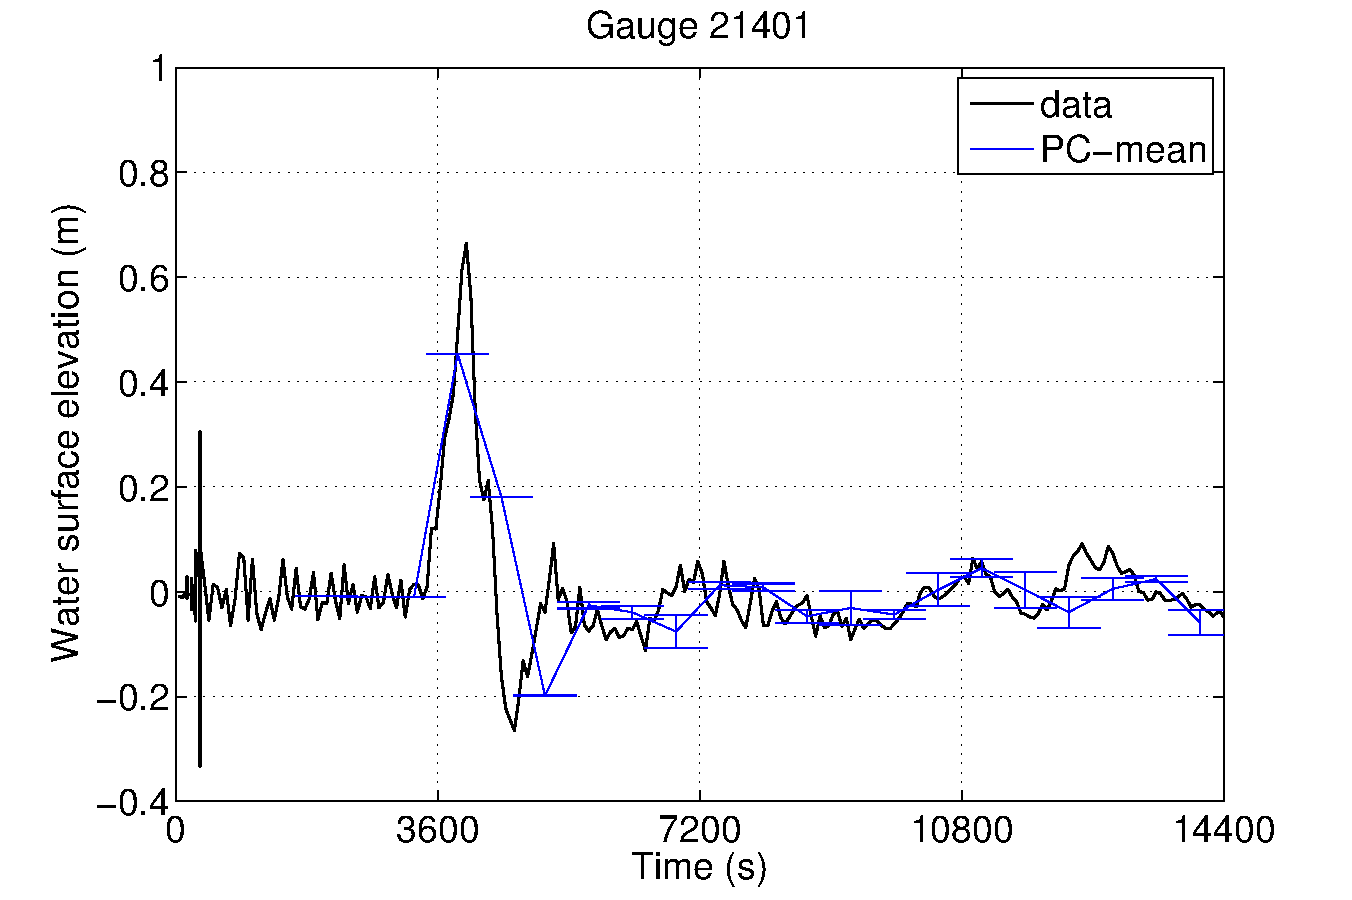
\includegraphics[width=0.475\textwidth]{./figures/compare1.pdf} &
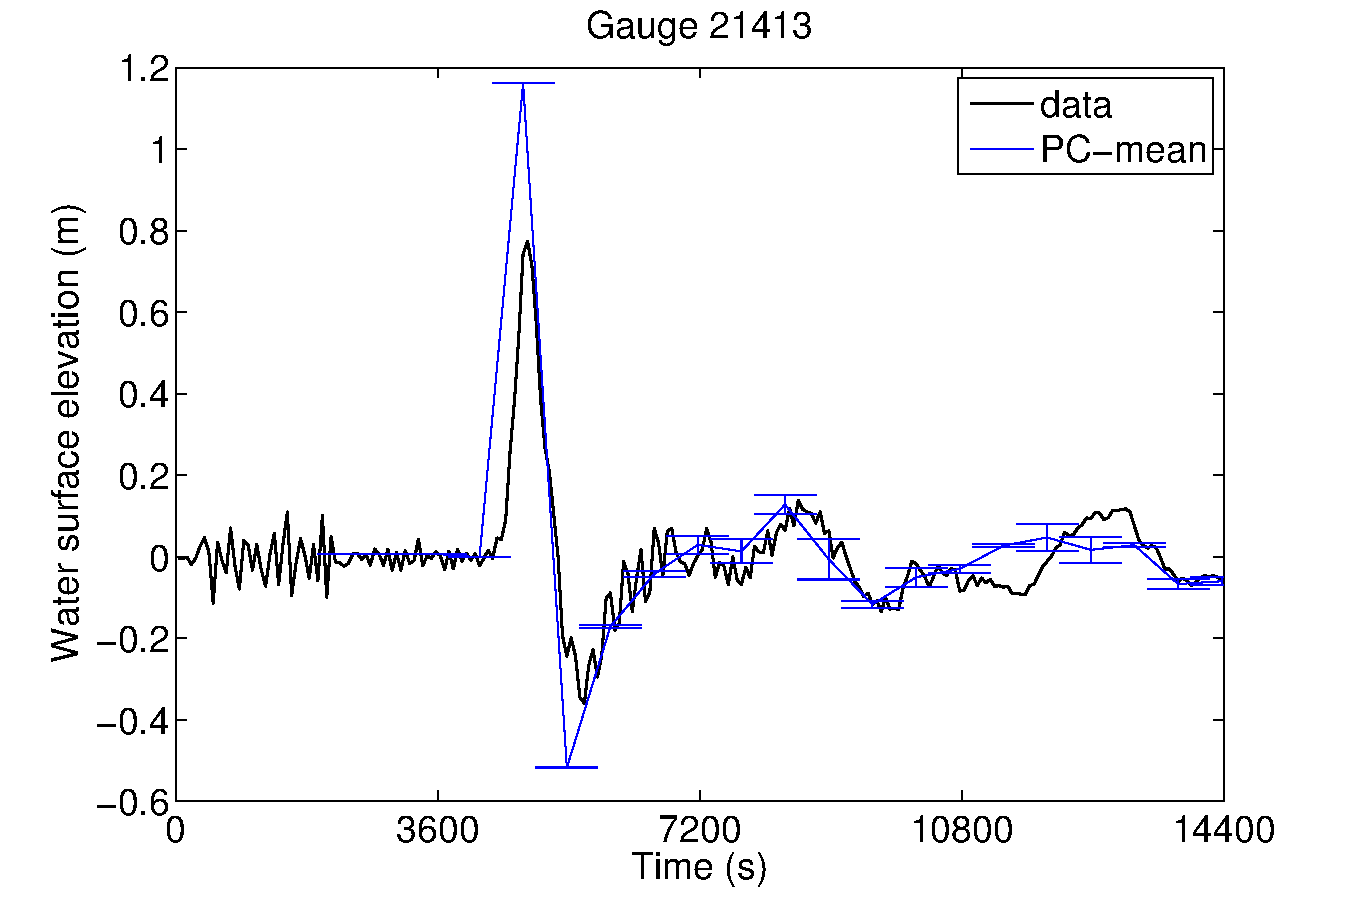
\includegraphics[width=0.475\textwidth]{./figures/compare2.pdf} \\
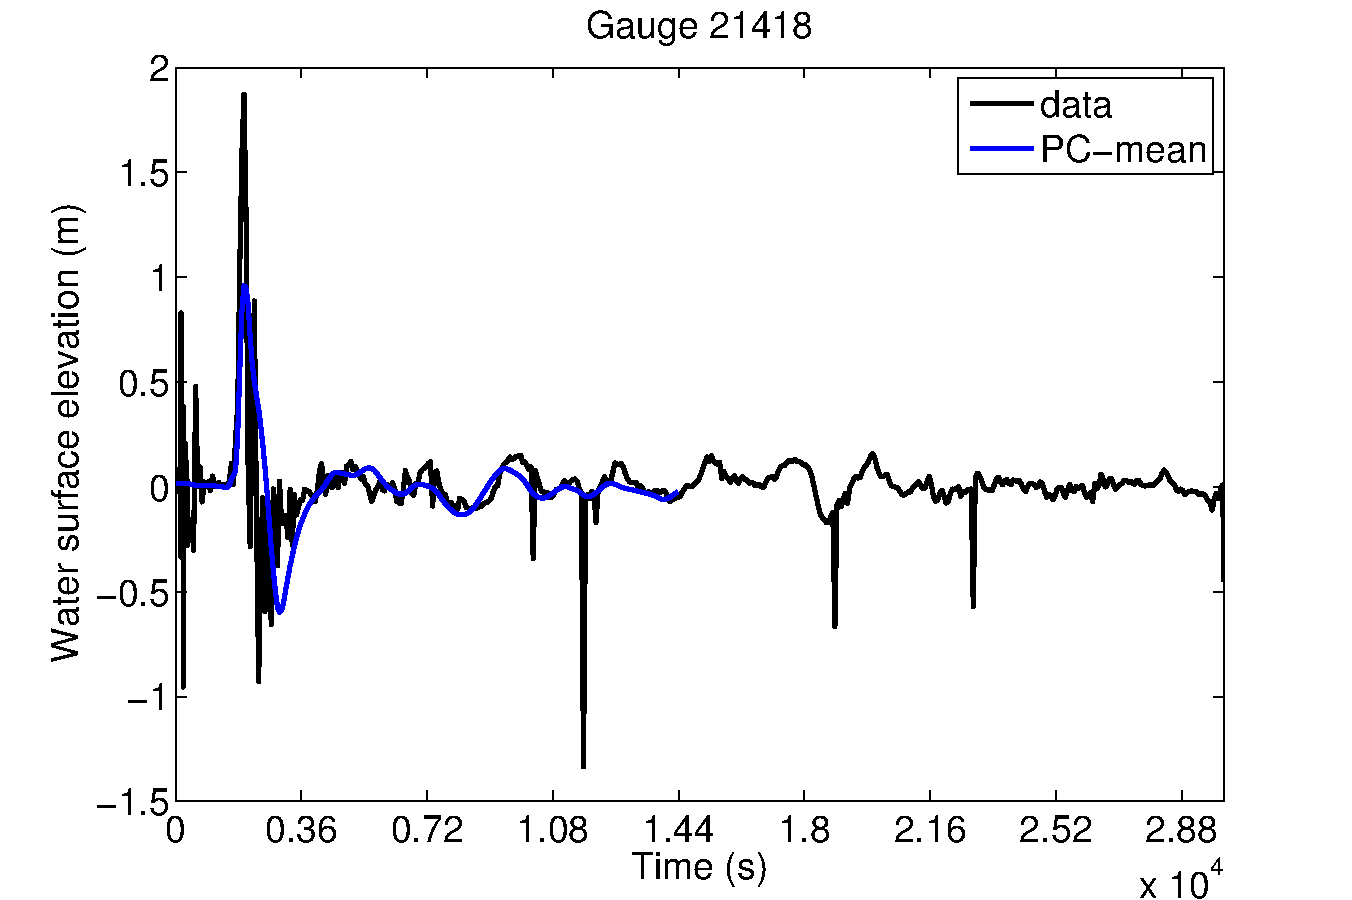
\includegraphics[width=0.475\textwidth]{./figures/compare3.pdf} &
\includegraphics[width=0.475\textwidth]{./figures/compare4.pdf}
\end{tabular}
\caption{Comparison of PC mean 
and observed data of water surface elevation with time at the four gauges.}
\label{fig:compare}
\end{figure}  
%%%%%%%%%%%%%%%%%%%%%%%%%%%%%%%%%%%%%%%%%%%%%%%%%%%%%%%%%%%%%%%%
\begin{figure}[h]
\centering
\includegraphics[width=0.475\textwidth]{./figures/scatter.pdf} 
\caption{Scatter plot of PC mean water surface elevation vs. observed ones.}
\label{fig:scatter}

\end{figure}  
%%%%%%%%%%%%%%%%%%%%%%%%%%%%%%%%%%%%%%%%%%%%%%%%%%%%%%%%%%%%%%%%
\begin{figure}[h]
\begin{tabular}{clc}
\includegraphics[width=0.475\textwidth]{./figures/chain_p1.pdf} &
\includegraphics[width=0.475\textwidth]{./figures/chain_p2.pdf} \\
\includegraphics[width=0.475\textwidth]{./figures/chain_p3.pdf} &
\includegraphics[width=0.475\textwidth]{./figures/chain_s1.pdf}
\end{tabular}
\caption{Chain samples for the three Manning's roughness coefficients $N_1,N_2,N_3$ and $\sigma^2$
the variance between simulations and observations.}
\label{fig:mcmc} 
\end{figure}
%%%%%%%%%%%%%%%%%%%%%%%%%%%%%%%%%%%%%%%%%%%%%%%%%%%%%%%%%%%%%%%%
 \begin{figure}[h]
        \begin{tabular}{clc}
\includegraphics[width=0.475\textwidth]{./figures/pdf_p1.pdf} &
\includegraphics[width=0.475\textwidth]{./figures/pdf_p2.pdf} \\
\includegraphics[width=0.475\textwidth]{./figures/pdf_p3.pdf} &
\includegraphics[width=0.475\textwidth]{./figures/pdf_s1.pdf}
        \end{tabular}
        \caption{Posterior distributions for the three Manning's roughness coefficients $N_1,N_2,N_3$ 
and $\sigma^2$ the variance between simulations and observations.}
\label{fig:pdfs} 
        \end{figure}
